\documentclass[ma3408.tex]{subfiles}

\begin{document}
\chapter{Bundle theory}
\section{Locally trivial bundles}
We begin with what we will call a locally trivially bundle.\footnote{Confusingly, some books will also call this a fiber bundle. We will see why later.}
\begin{Def}
A map $\pi \colon E\to B$ is a locally trivial bundle with fiber $F$ if the following conditions hold:
\begin{enumerate}
	\item Each point $b \in B$ has a neighborhood $U$ such that $\pi^{-1}(U_b) \xrightarrow{h_b} U_b \times F$.
	\item The following diagram commutes
	% https://q.uiver.app/?q=WzAsMyxbMCwwLCJcXHBpXnstMX0oVV9iKSJdLFsyLDAsIlVfYiBcXHRpbWVzIFxccGleey0xfShiKSJdLFsxLDEsIlVfYiJdLFswLDEsImhfYiJdLFswLDIsIlxccGkiLDJdLFsxLDIsIlxcdGV4dHtwcn1fMSJdXQ==
\[\begin{tikzcd}[ampersand replacement=\&]
	{\pi^{-1}(U_b)} \&\& {U_b \times F} \\
	\& {U_b}
	\arrow["{h_b}", from=1-1, to=1-3]
	\arrow["\pi"', from=1-1, to=2-2]
	\arrow["{\text{pr}_1}", from=1-3, to=2-2]
\end{tikzcd}\]
\end{enumerate}
The maps $h_b$ are called the \emph{local trivializations} of the bundle.
\end{Def}
\begin{Exa}
Let $E = B \times F$ and $\pi \colon E  = B \times F \to B$ the projection map. This is called the trivial bundle. 
\end{Exa}
\begin{Exa}
If $F$ is discrete, then a locally trivial bundle with fiber $F$ is a covering map. 
\end{Exa}
\begin{Exa}\label{exa:mobius}
The M{\"o}bius band is a locally trivial bundle with fiber $S^1$, see \Cref{fig:mob}. 
\begin{figure}[h!] \centering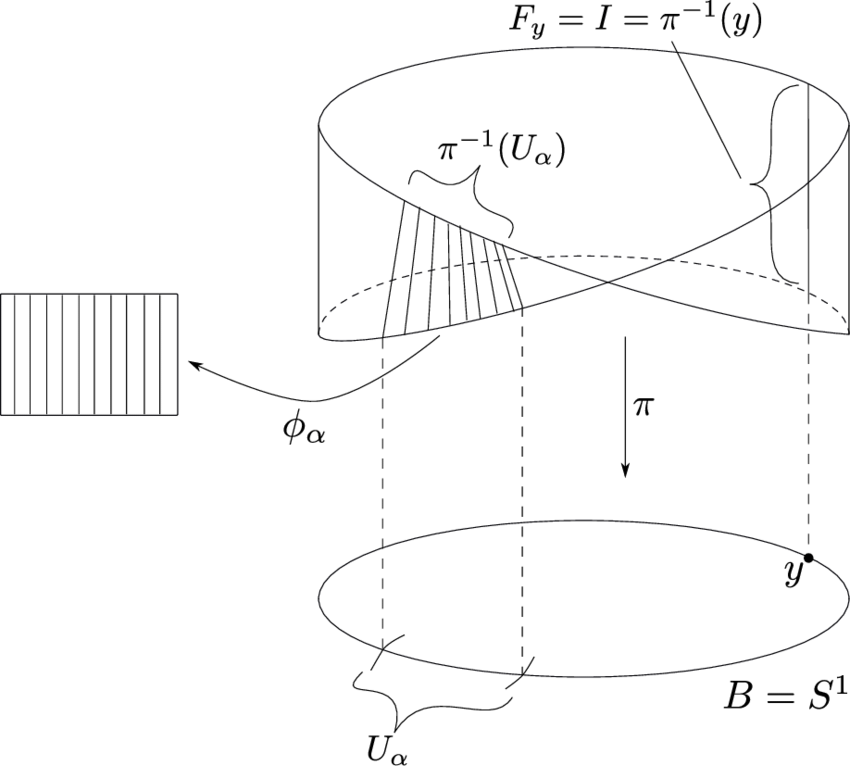
\includegraphics[scale = 0.25]{mob.png}\caption{The M{\"o}bius band}\label{fig:mob}\end{figure}
We will return to this example in due course. 
\end{Exa}
\begin{Rem}\label{rem:fibration-serre}
We can write a locally trivial bundle as $F \to E \to B$, which is reminiscent of the notation for a fibration. In fact, fiber bundles over paracompact base spaces are always fibrations.\footnote{A space is paracompact if every open cover has an open refinement that is locally finite. } More generally, any locally trivial bundle is a Serre fibration. 
\end{Rem}
\begin{Rem}
Let us unwind the definition of a locally trivial bundle a little more. Let $\pi \colon E \to B$ be a locally trivial bundle with fiber $F$. From the definition we can cover $B$ by a family of open sets $\{ U_{\alpha} \}$ such that each inverse image $\pi^{-1}(U_{\alpha})$ is fiberwise homeomorphic to $U_{\alpha} \times F$ . This gives a system of homeomorphisms
\[
\phi_{\alpha} \colon U_{\alpha} \times F \to \pi^{-1}(U_{\alpha}). 
\]
Observe that if $V \subseteq U_{\alpha}$ then the restriction of $\phi_{\alpha}$ to $V \times F$ gives the homeomorphism with $\pi^{-1}(V)$. Hence on $U_{\alpha} \cap U_{\beta}$ there are two fiberwise homeomorphisms
\[
\begin{split}
\phi_{\alpha} &\colon (U_{\alpha} \cap U_{\beta})\times F \to \pi^{-1}(U_{\alpha} \cap U_{\beta})\\
\phi_{\beta} &\colon (U_{\alpha} \cap U_{\beta})\times F \to \pi^{-1}(U_{\alpha} \cap U_{\beta})
\end{split}
\]
Consider the following commutative diagram
% https://q.uiver.app/?q=WzAsNCxbMCwwLCIoVV97XFxhbHBoYX0gXFxjYXAgVV97XFxiZXRhfSkgXFx0aW1lcyBGIl0sWzEsMCwiXFxwaV57LTF9KFVfe1xcYWxwaGF9IFxcY2FwIFVfe1xcYmV0YX0pIl0sWzIsMCwiKFVfe1xcYWxwaGF9IFxcY2FwIFVfe1xcYmV0YX0pIFxcdGltZXMgRiJdLFsxLDEsIlVfe1xcYWxwaGF9IFxcY2FwIFVfe1xcYmV0YX0iXSxbMCwxLCJcXHBoaV97XFxhbHBoYX0iXSxbMSwyLCJcXHBoaV97XFxiZXRhfV57LTF9Il0sWzEsM10sWzAsM10sWzIsM11d
\[\begin{tikzcd}[ampersand replacement=\&]
	{(U_{\alpha} \cap U_{\beta}) \times F} \& {\pi^{-1}(U_{\alpha} \cap U_{\beta})} \& {(U_{\alpha} \cap U_{\beta}) \times F} \\
	\& {U_{\alpha} \cap U_{\beta}}
	\arrow["{\phi_{\alpha}}", "\cong"', from=1-1, to=1-2]
	\arrow["{\phi_{\beta}^{-1}}", "\cong"',from=1-2, to=1-3]
	\arrow[from=1-2, to=2-2]
	\arrow[from=1-1, to=2-2]
	\arrow[from=1-3, to=2-2]
\end{tikzcd}\]
Let $\phi_{\alpha\beta}$ denote the top composite $\phi_{\beta}^{-1}\phi_{\alpha}$. Then the locally trivially bundle is completed determined by the base $B$, the fiber $F$, the covering $U_{\alpha}$ and the homeomorphisms $U_{\alpha\beta}$. Roughly speaking, $E$ should be thought of as the cartesian product of the $U_{\alpha} \times F$ with some identifications by the $\phi_{\alpha\beta}$. 
\end{Rem}
\begin{Def}
The open sets $U_{\alpha}$ are called \emph{charts}, the family $U_{\alpha}$ the \emph{atlas of charts}, the homeomorphisms $\phi_{\alpha}$ are called the \emph{coordinate homeomorphisms} and the $\phi_{\alpha\beta}$ are called the \emph{transition functions.}
\end{Def}
\begin{Rem}\label{rem:bundle_construction}
In order for homeomorphisms $\phi_{\alpha\beta}$ to be the transition functions of a locally trivial bundle, they must satisfy a number of conditions. For example,
\[
\phi_{\alpha\alpha} = \text{id} 
\]
and
\[
 \phi_{\gamma\alpha}\phi_{\beta\gamma}\psi_{\alpha\beta} = \text{id}
\]
on any triple $(U_{\alpha} \cap U_{\beta} \cap U_{\gamma}) \cap F$. Taking $\gamma = \alpha$ we get
\[
\phi_{\alpha\beta}\phi_{\beta\alpha} = \text{id}.
\]
In fact, these conditions suffices to reconstruct the locally trivial bundle for the base, the fiber, atlas and homeomorphisms. Indeed, set $E = E'/\sim$ where
\[
E' = \bigcup_{\alpha} (U_{\alpha} \times F)
\]
and for $(x,f) \in U_{\alpha} \times F$ and $(y,g) \in U_{\beta} \times F$ we have $(x,f) \sim (y,g) \iff x = y \in (U_{\alpha} \cap U_{\beta})$ and $(y,g) = \phi_{\alpha\beta}(x,f)$. It is a rather tedious exercise to show that this determines a locally trivial bundle. 
\end{Rem}
\begin{Def}
Two locally trivial bundles $\pi \colon E \to B$ and $\pi' \colon E' \to B'$ are isomorphic if there is a homeomorphism $\psi \colon E \to E'$ such that the diagram
% https://q.uiver.app/?q=WzAsMyxbMCwwLCJFIl0sWzIsMCwiRSciXSxbMSwxLCJGIl0sWzAsMSwiXFxwc2kiXSxbMCwyLCJcXHBpIiwyXSxbMSwyLCJcXHBpJyJdXQ==
\[\begin{tikzcd}[ampersand replacement=\&]
	E \&\& {E'} \\
	\& B
	\arrow["\psi", from=1-1, to=1-3]
	\arrow["\pi"', from=1-1, to=2-2]
	\arrow["{\pi'}", from=1-3, to=2-2]
\end{tikzcd}\]
commutes. (Note that this implies that there is a homeomorphism $F \to F'$ between the fibers as well).
\end{Def}
\begin{Thm}
Two systems of transition functors $\phi_{\beta\alpha}$ and $\phi_{\beta\alpha}'$ define isomorphic locally trivial bundles iff there exists fiber preserving homeomorphisms
\[
h_{\alpha} \colon U_{\alpha} \times F \to U_{\alpha} \times F
\]
such that $\phi_{\beta\alpha}= h_{\beta}^{-1}\phi'_{\beta\alpha}h_{\alpha}$. 
\end{Thm}
\begin{proof}
First, we suppose that the two bundles are isomorphic, so in particular there is a homeomorphism $\psi \colon E \to E'$. We let 
\[h_{\alpha} \coloneqq \phi_{\alpha}^{'-1}\psi^{-1}\phi_{\alpha}\colon U_{\alpha} \times F \to U_{\alpha} \times F. 
\]
Then we have
\[
\begin{split}
h_{\beta}^{-1}\phi'_{\beta\alpha}h_{\alpha} &= \phi_{\beta}^{-1}\psi^{-1}\phi'_{\beta}\phi'_{\beta\alpha}\phi_{\alpha}^{-1}\psi^{-1}\phi_{\alpha}\\
&=\phi_{\beta}^{-1}\psi^{-1}\phi_{\beta'}\phi_{\beta}^{'-1}\phi'_{\alpha}\phi_{\alpha}^{-1}\psi^{-1}\phi_{\alpha} = \phi_{\beta\alpha}.
\end{split}
\]
Conversely, if the relations hold, then we set $\psi = \phi_{\alpha}h_{\alpha}^{-1}\phi^{'-1}_{\alpha}$. A similar argument then shows that $\phi_{\beta}h_{\beta}^{-1}\phi^{'-1}_{\beta} = \phi_{\alpha}h_{\alpha}^{-1}\phi{'-1}_{\alpha}$. 
\end{proof}
\begin{Rem}\label{rem:not_a_trivial_bundle}
If $\pi$ is (isomorphic to) a trivial bundle, then all transition functions can be chosen to be the identity. One can use the previous theorem to show that a bundle is not isomorphic to a trivial bundle. 
\end{Rem}
\begin{Exa}\label{exa:mobius2}
After this discussion, let us return to the example of the M{\"o}bius bundle (\Cref{exa:mobius}). One can think of this as the space
\[
E = \{(x,y) \colon 0 \le x \le 1, 0 \le y \le 1 \}/\sim
\]
where we identify $(0,y)$ and $(1,1-y)$ for each $y \in [0,1]$. The projection maps $E$ to $I_x =\{ 0 \le x \le 1\}$ with the endpoints identified, that is, onto the circle. To see that this is a bundle we use the atlas
\[
U_{\alpha} = \{ 0 \le x \le 1 \}, \text{ and } U_{\beta} = \{ 0 \le x < 1/2\} \cup \{ 1/2 < x \le 1 \}. 
\]
We define
\[
\phi_{\alpha} \colon U_{\alpha} \times I_y \to E, \quad \phi_{\alpha}(x,y) = (x,y), 
\]
and
\[
\phi_{\beta} \colon U_{\beta} \times I_y \to E
\]
by
\[
\phi_{\beta} = \begin{cases}(x,y) & \text{for } 0 \le x \le /1/2, \\ (x,1-y) & \text{for } 1/2 < x \le 1.\end{cases}
\]
The intersection of these two charts is the union $(0,1/2) \cup (1/2,1)$, and the transition functions have the form
\[
\phi_{\beta\alpha} = (x,y) \text{ for } 0 < x < 1/2
\]
and 
\[
\phi_{\beta\alpha} = (x,1-y) \text{ for } 1/2 < x < 1.
\]
One can check from \Cref{rem:not_a_trivial_bundle} that the M{\"o}bius bundle is not isomorphic to a trivial bundle. 
\end{Exa}
We now give some more examples which will be useful in our study of characteristic classes. 
\begin{Def}
For $n<k$ the $n$-th Stiefel manifold associated to $\bbR^k$ is defined as
\[
V_n(\bbR^k) = \{ n-\text{frames in } \bbR^k \}
\]
where an $n$-frame in $\bbR^k$ is a tuple $\{v_1,\ldots,v_n\}$	of orthonormal vectors in $\bbR^k$, i.e., $v_1,\ldots,v_n$ are pairwise orthonormal, $\langle v_i,v_j \rangle = \delta_{ij}$. We given $V_n(\bbR^k)$ the subspace topology induced by thinking of it as a subspace of $S^{k-1} \times \ldots S^{k-1}$ ($n$-copies of $S^{k-1}$). 
\end{Def}
\begin{Exa}
A 1-frame is nothing but a unit vector, so the Stiefel manifold $V_1(\bbR^k)$ is the unit sphere in $\bbR^k$, i.e., $V_1(\bbR^k) \cong S^{k-1}$. On the other hand, an $n$-frame is an ordered basis, so $V_n(\bbR^n) \cong O(n)$. 
\end{Exa}
\begin{Def}
The $n$-th Grassmannian associated to $\bbR^k$ is defined as 
\[
G_n(\bbR^k) = \{ n-\text{dimensional vector subspaces in } \bbR^k \}
\]
There is a map $p \colon V_n(\bbR^k) \to G_n(\bbR^k)$ sending $\{ v_1,\ldots,v_n\}$ to the span, which is surjective by Gram--Schmidt, and we given $G_n(\bbR^k)$ the quotient topology. 
\end{Def}
\begin{Exa}
We have $G_1(\bbR^k)$ is the space of lines through the origin in $k$-space, so $G_1(\bbR^k) \simeq \bbR P^{k-1}$.
\end{Exa}
\begin{Lem}
	For $k>n$ the quotient map $p \colon V_n(\bbR^k) \to G_n(\bbR^k)$ is a locally trivial bundle with fiber $V_n(\bbR^n) \cong O(n)$, i.e., we have a locally trivial bundle
	\begin{equation}\label{eq:fiber-bundle-vn-gn}
	O(n) \to V_n(\bbR^k) \xrightarrow{p} G_n(\bbR^k). 
	\end{equation}
	Similarly, for $m <n \le k$ there are locally trivial bundles 
		\begin{equation}\label{eq:fiber-bundle-vn-vm}
	V_{n-m}(\bbR^k) \to V_n(\bbR^k) \xrightarrow{p} V_m(\bbR^k). 
	\end{equation}
	where the map $p$ takes $\{ v_1,\ldots,v_n\}$ to $\{ v_1,\ldots,v_m \}$. Taking $k =n$ we get a locally trivial bundle
			\begin{equation}\label{eq:fiber-bundle-on-vm}
	O(n-m) \to O(n) \xrightarrow{p} V_m(\bbR^n). 
	\end{equation}
\end{Lem}
\begin{Exa}
Taking $m = 1$ in \eqref{eq:fiber-bundle-on-vm} we get a locally trivial bundle
\[
O(n-1) \to O(n) \to S^{n-1}.
\]
Here the first map takes $A$ to $ \begin{pmatrix}
A & 0 \\
0 & 1 
\end{pmatrix}  $ and the second takes $B$ to $Bu$ for $u \in S^{n-1}$ some unit vector. In particular, this identifies $S^{n-1}$ as an orbit space $S^{n-1} \cong O(n)/O(n-1)$. 
\end{Exa}
\begin{exercise}
Use the fibrations
\[
O(n-k) \to O(n) \to V_k(\mathbb{R}^n)
\]
to show that
\[
\pi_i(O(n-1)) \simeq \pi_i(O(n)) \text{ for } i < n-2
\]
and
\[
\pi_i(V_k(\mathbb{R}^n)) = 0
\]
for $i < n-k-1$. 
\end{exercise}
\begin{Def}
We have infinite versions of the Stiefel manifold and Grassmanian:
\[
V_n(\bbR^{\infty}) \coloneqq \bigcup_{k=1}^{\infty} V_n(\bbR^k) \quad \quad G_n(\bbR^{\infty}) \coloneqq \bigcup_{k=1}^{\infty} G_n(\bbR^k)
\]
\end{Def}
\begin{Rem}
We get a fiber sequence 
\[
O(n) \to V_n(\bbR^{\infty}) \to G_n(\bbR^{\infty}).
\]
\end{Rem}

\begin{Prop}
$V_n(\bbR^{\infty})$ is contractible.
\end{Prop}
\begin{proof}
	As in the exercise, we deduce that $\pi_i(V_n(\bbR^{\infty}) = 0$ for all $i$. We can give $V_n(\bbR^{\infty})$ the structure of a CW-complex, and so the claim follows from \Cref{cor:contractible_cw}. 
\end{proof}
\begin{Rem}
One can repeat the same story using $\bbC$ or $\mathbb{H}$ instead of $\bbR$. In the first case, all instances of $O(n)$ get replaced by $U(n)$, and in the second case by $\Sp(n)$. 
\end{Rem}
\begin{Exa}[The tangent bundle to {$S^2$}]\label{exa:ts2}
Let $S^2 = \{ (x_0,x_1,x_2) \in \bbR^3 \mid x_0^2+x_1^2+x_2^2 = 1\}$. Recall that the tangent space at a point $x \in S^2$ is defined by $T_xS^2 = \{\xi \in \bbR^3 \mid x \bot \xi \}$. We then define $TS^2 = \coprod_{x \in S^2}T_xS^2$. This can be topologized as a subspace of $\bbR^3 \times \bbR^3$ when we write
\[
TS^2 = \{ (x,\xi) \in \bbR^3 \times \bbR^3 \mid x \in S^2, x \bot \xi \}.
\]
There is a natural projection map $p \colon TS^2 \to S^2$ sending the pair $(x,\xi)$ to $x$, which we claim is a locally trivial bundle with fiber $\bbR^2$.  To see this is a locally trivial bundle, let $U$ be the open subset of $S^2$ defined by $x_3>0$. We will show how to construct the local trivialization on this open subset. 

If $\xi = (\xi_1,\xi_2,\xi_3)$ then we have the relation
\[
x_1\xi_1 + x_2\xi_2 + x_3\xi_3 = 0
\]
or 
\[
\xi_3 = -(x_1\xi_1 + x_2\xi_2)/x_3.
\]
We define
\[
\phi \colon U \times \bbR^2 \to p^{-1}(U)
\]
by
\[
\phi(x_1,x_2,x_3,\xi_1,\xi_2) = (x_1,x_2,x_3,\xi_1,\xi_2,-(x_1\xi_1 + x_2\xi_2)/x_3),
\]
which gives the required chart for this open subset. 
\end{Exa}
\begin{Rem}
More generally, for any smooth manifold $X$ of dimension  $n$, we have a locally trivial bundle $\pi \colon TX \to X$ with fiber $\bbR^n$. 
\end{Rem}
\section{The structure group of locally trivial bundles}
We recall that the on the intersection of two local trivializations we constructed a homeomorphism
\[
\phi_{\beta\alpha} \colon {(U_{\alpha} \cap U_{\beta}) \times F} \to {\pi^{-1}(U_{\alpha} \cap U_{\beta})} \to {(U_{\alpha} \cap U_{\beta}) \times F} 
\]
Unwinding the definition, the map $\phi$ is completely determine by a map  $\Phi \colon U \to \Homeo(F)$, where $\Homeo(F)$ denotes the group of all homeomorphisms of the fiber $F$ (we call $ \Phi$ coordinate transformations).\sidenote{If we choose the correct topology on $\Homeo(F)$, namely the compact-open topology (for reasonable spaces at least), then this map is even continuous}. Indeed, we have
\[
\phi_{\alpha\beta}(x,f) = (x,\Phi(x)(f))
\]
In other words, instead of $\phi_{\alpha\beta}$ to determine a bundle we can instead specify a family of functions
\[
\Phi_{\alpha\beta}(x,f) \colon U_{\alpha} \cap U_{\beta} \to \Homeo(F),
\]
having values in the group $\Homeo(F)$. Of course these are not arbitrary, but need to satisfy various compatibility conditions:
\[
\Phi_{\alpha\alpha}(x) = \text{id} 
\]
and 
\[
\Phi_{\alpha\gamma}(x)\Phi_{\gamma\beta}(x)\Phi_{\beta\alpha}(x) = \text{id},
\]
for $x \in U_{\alpha} \cap U_{\beta} \cap U_{\gamma}$.
\begin{Def}
Let $E,B,F$ be topological spaces and $G$ a topological group which acts freely on the space $F$. A continuous map $p \colon E \to B$ is a locally trivial bundle with fiber $F$ and structure group $G$ if there is an atlas $\{ U_{\alpha} \}$ and the coordinate homeomorphisms
\[
\phi_{\alpha} \colon U_{\alpha} \times F \to p^{-1}(U_{\alpha})
\]
such that the transition functions
\[
\phi_{\beta\alpha} = \phi_{\beta}^{-1}\phi_{\alpha} \colon (U_{\alpha} \cap U_{\beta}) \times F \to (U_{\alpha} \cap U_{\beta}) \times F
\]
have the form
\[
\phi_{\beta\alpha}(x,f) = (x,\Phi_{\beta\alpha}(x)f)
\]
where $\Phi_{\beta\alpha} \colon (U_{\alpha} \cap U_{\beta}) \to G$ are continuous functions satisfying 
\[
\Phi_{\alpha\alpha}(x) = \text{id} 
\]
and 
\[
\Phi_{\alpha\gamma}(x)\Phi_{\gamma\beta}(x)\Phi_{\beta\alpha}(x) = \text{id},
\]
\end{Def}
\begin{Rem}
Some words on terminology are useful. What we defined as a locally trivial bundle with fiber $F$, is exactly a locally trivial bundle with fiber $F$ and structure group $\Homeo(F)$. Either of these may also be called a \emph{fiber bundle} or a \emph{fiber bundle with structure group $G$.}
\end{Rem}
\begin{Rem}
In diagrammatic form, to have structure group $G$ means that we can find transition maps $\Phi'_{\alpha\beta}$ making the diagram commute:
% https://q.uiver.app/?q=WzAsMyxbMiwwLCJcXEhvbWVvKEYpIl0sWzEsMSwiVV97XFxhbHBoYX0gXFxjYXAgVV97XFxiZXRhfSJdLFswLDAsIkciXSxbMSwwLCJcXG92ZXJsaW5le1xccGhpfV97XFxhbHBoYVxcYmV0YX0iLDJdLFsyLDBdLFsxLDIsIlxcb3ZlcmxpbmV7XFxwaGl9J197XFxhbHBoYVxcYmV0YX0iLDAseyJzdHlsZSI6eyJib2R5Ijp7Im5hbWUiOiJkYXNoZWQifX19XV0=
\[\begin{tikzcd}[ampersand replacement=\&]
	G \&\& {\Homeo(F)} \\
	\& {U_{\alpha} \cap U_{\beta}}
	\arrow["{\Phi_{\alpha\beta}}"', from=2-2, to=1-3]
	\arrow[from=1-1, to=1-3]
	\arrow["{\Phi'_{\alpha\beta}}", dashed, from=2-2, to=1-1]
\end{tikzcd}\]
\end{Rem}
\begin{Rem}
Note that the structure group is not unique. For example, a bundle with structure group $G$ may admit transition functions with values in a subgroup $H \le G$. We say that the structure group $G$ is reduced to subgroup $H$. More generally, if $\rho \colon G \to G'$ is a continuous homeomorphism of topological groups, and we are given a locally trivial bundle with structure group $G$ and the transition functors $\alpha_{\alpha \beta} \colon U_{\alpha} \cap U_{\beta} \to G$ , then a new locally trivial bundle with structure group $G'$ may be constructed by 
\[
\phi'_{\alpha\beta}(x) = \rho(\phi_{\alpha\beta}(x)).
\]
This operation is called the change of structure group. 
\end{Rem}
\begin{exercise}
Show that a trivial bundle has trivial structure group. Conversely, if the structure group can be reduced to the trivial group then the bundle is (isomorphic to) a trivial bundle. 
\end{exercise}
\begin{Exa}
Let us return to the M{\"o}bius bundle (\Cref{exa:mobius,exa:mobius2}). We have that 
\[
\Phi_{\alpha\beta}(y) = y \quad \text{ and } \Phi_{\beta\alpha}(y) = 1-y.
\]
Note that $\Phi_{\beta\alpha} \circ \Phi_{\beta\alpha}(y) = 1-(1-y) = y = \Phi_{\alpha\beta}(y)$. Therefore, the group generated by $\Phi_{\alpha\beta}$ and $\Phi_{\beta\alpha}$ has order 2. In other words, the M{\"o}bius bundle has (or can be reduced to) structure group $\bbZ/2$. 
\end{Exa}
\begin{Exa}
The tangent bundle $TS^2 \to S^2$ was considered in \Cref{exa:ts2}. The coordinate homeomorphisms
\[
\phi \colon U \times \bbR^2 \to \bbR^3 \times \bbR^3
\]
are defined by formulas that are linear with respect to the second argument. Hence that transition functions have values in the group of linear translations of the fiber $F = \bbR^2$, that is $G = GL_2(\bbR)$. In fact, it can be shown that the structure group can be reduced to the subgroup $O(n)$ of orthonormal rotations. 
\end{Exa}
\section{Principal bundles}
The most important example of a bundle for a us is a \emph{principal bundle}. We postpone the definition to talk a little about group actions. 
\begin{Def}
Let $G$ be a topological group, and $X$ a topological space. A left action of $G$ on $X$ is a continuous map $\mu \colon G \times X \to X$, satisfying $\mu(e,x) = x$ and $\mu(h,\mu(g,x)) = \mu(hg,x)$. 
\end{Def}
\begin{Exa}
The multiplication map $\mu \colon G \times G \to G$ defines a left action of $G$ on itself. Similarly, if $H \subseteq G$, then $\mu|_{H \times G} \colon H \times G \to G$ defines an action of $H$ on $G$. 
\end{Exa}
\begin{Rem}
The map $\mu \colon G \times X \to X$ is adjoint to a map $ad(u) \colon G \to \Homeo(X)$, where $\Homeo(X)$ has the compact-open topology. If $X$ is nice (specifically, locally compact Hausdorff) then a continuous map $G \to \Homeo(X)$ gives rise to a group action $G \times X \to X$. 
\end{Rem}
\begin{Exa}\label{exa:adjoint_top_group}
The adjoint to the multiplication $\mu \colon G \times G \to G$ is the map $G \to \Homeo(G)$ given by $g \mapsto f_g$, where $f_g \colon G \to G$ is given by $f_g(x) = gx$.  
\end{Exa}
\begin{Rem}
We recall some standard terminology associated to a group action of $G$ on $X$:
\begin{enumerate}[(i)]
	\item The orbit of a point $x \in X$ is the set $Gx = \{ g \cdot x mid g \in G \}$. 
	\item The orbit space $X/G$ is the quotient space $X/\sim$ where $x \sim g \cdot x$. 
	\item The fixed set $X^G \coloneqq \{ x \in X | g \cdot x \text{ for all } g \in G \}$. 
	\item An action if free\sidenote{Here, meaning fixed-point free} if $g \cdot x \ne x$ for all $x \in X$ and all $g \ne e$. (i.e., $gx = x$ for all $x$ implies $g = e$). 
	\item The stabilizer (or isotropy) group at $x$ is $G_x = \{ g \in G \mid g\cdot x = g \} \subseteq G$. 
	\item An action is effective is the adjoint $G \to \Homeo(X)$ is injective, or equivalently if $\cap_{x \in X} G_x = \{ e \}$.\sidenote{Note that a free action is effective, but not vice-versa.}
	\item A group action is transitive if and only if it has exactly one orbit, i.e., there exists $x \in X$ such that $Gx = X$. 
\end{enumerate}
\end{Rem}
\begin{Exa}\label{exa:hopf_bundle}
To motivate the definition of a principal $G$-bundle we first consider an example. We recall that Hopf fibration $S^1 \to S^3 \to S^2$. By what we have already discussed, this is a locally trivial bundle. 

 Let us show this directly. Consider the sphere $S^3$ as a subset of $\mathbb{C}^2$ defined by the equation
\[
|z_0|^2 + |z_1|^2 = 1.
\]
Then the map $S^3 \to S^2 = \mathbb{C}P^1$ sends $(z_0,z_1)$ to the projective coordinate $[z_0 : z_1]$. We take the atlas consisting of the charts
\[
\begin{split}
U_0 &= \{ [z_0,z_1] : z_0 \ne 0\}\\
U_1 &= \{ [z_0,z_1] : z_1 \ne 0\}
\end{split}
\]
The points of the chart $U_0$ are parametrized by the complex parameter $w_0 = z_1/z_0 \in \mathbb{C}$, while points of the chart $U_1$ are parameterized by $w_1 = z_0/z_1 \in \mathbb{C}$. The homeomorphisms
\[
\phi_0 \colon p^{-1}(U_0) \to S^1 \times \bbC = S^1 \times U_0 \text{ and }\phi_0 \colon p^{-1}(U_1) \to S^1 \times \bbC = S^1 \times U_1
\]
are given by
\[
\begin{split}
\phi_0(z_0,z_1) &= \left(\frac{z_0}{|z_0|},\frac{z_1}{z_0}\right) = \left(\frac{z_0}{|z_0|},[z_0 : z_1]\right)\\
\phi_0(z_0,z_1) &= \left(\frac{z_1}{|z_1|},\frac{z_0}{z_1}\right) = \left(\frac{z_1}{|z_1|},[z_0 : z_1]\right)
\end{split}
\]
One can explicitly write down inverses for these maps and check that they are homeomorphisms. The transition function
\[
\phi_{01} \colon (U_0 \cap U_1) \times S^1 \to (U_0 \cap U_1)\times S^1  
\]
is defined by the formula
\[
\phi_{01}([z_0:z_1],\lambda) = \left([z_0:z_1],\frac{z_1|z_0|}{z_0|z_1|}\right).
\]
In other words, $\Phi_{01} \colon U_0 \cap U_1 \to \Homeo(S^1)$ is defined by 
\[
[z_0:z_1] \mapsto (\lambda \mapsto \frac{z_1|z_0|}{z_0|z_1|}\lambda),
\]
where $\frac{z_1|z_0|}{z_0|z_1|} \in S^1$. We can then define a map $\Phi'_{01} \colon U_0 \cap U_1 \to S^1$ by $[z_0,z_1] \mapsto \frac{z_1|z_0|}{z_0|z_1|}$. Unwinding the definitions, the diagram
% https://q.uiver.app/?q=WzAsMyxbMCwwLCJTXjEiXSxbMiwwLCJcXEhvbWVvKFNeMSkiXSxbMSwxLCJVXzAgXFxjYXAgVV8xIl0sWzAsMSwiYWQoXFxtdSkiXSxbMiwwLCJcXG92ZXJsaW5le1xccGhpJ197MDF9fSJdLFsyLDEsIlxcb3ZlcmxpbmV7XFxwaGlfezAxfX0iLDJdXQ==
\[\begin{tikzcd}[ampersand replacement=\&]
	{S^1} \&\& {\Homeo(S^1)} \\
	\& {U_0 \cap U_1}
	\arrow["{ad(\mu)}", from=1-1, to=1-3]
	\arrow["{\Phi'_{01}}", from=2-2, to=1-1]
	\arrow["{\Phi_{01}}"', from=2-2, to=1-3]
\end{tikzcd}\]
commutes, where $ad(\mu)$ is adjoint to the multiplication map $\mu \colon S^1 \times S^1 \to S^1$.\sidenote{Here we use \Cref{exa:adjoint_top_group}.}

In other words, the structure group of the Hopf bundle can be reduced to $S^1$, where the action of $S^1$ on the fiber, namely $S^1$ again, is given by the multiplication map $\mu \colon S^1 \times S^1 \to S^1$. 

This leads us to the following definition. 
\end{Exa}
\begin{Def}
A locally trivial bundle with structure group $G$ is called a principal $G$-bundle if $F = G$ and the action of the group $G$ on $F$ is defined by left translations, i,e, the multiplication map $\mu \colon G \times G \to G$ as in \Cref{exa:adjoint_top_group}. 
\end{Def}
\begin{Exa}
Restated, \Cref{exa:hopf_bundle} shows that $S^1 \to S^3 \to S^2$ is a principal $S^1$-bundle. 
\end{Exa}
\begin{Thm}\label{thm:g-action-principal-bundles}
Let $p \colon E \to B$ be a principal $G$-bundle, with 
\[
\phi_{\alpha} \colon U_{\alpha} \times G \to p^{-1}(U_{\alpha})
\]
coordinate homeomorphisms. Then there is a \emph{right action}\sidenote{Why on the right? This is just because the action of $G$ on $E$ is given by \emph{left} translation. If we made the opposite convention, then $E$ would get a left action of $G$.} of the group $G$ on the total space $E$ such that 
\begin{enumerate}[(i)]
\item The right action is fiberwise,\sidenote{In other words, it preserves fibers.} i.e., $p(x) = p(xg)$ for $x \in E,g\in G$. 
\item The homeomorphism $\phi_{\alpha}^{-1}$ transformations the right action of the group $G$ on the total space into right translations on the second factor, i.e., 
\begin{equation}\label{eq:right_g_action}
\phi_{\alpha}(x,f)g = \phi_{\alpha}(x,fg), \hspace{2mm} x \in U_{\alpha},f,g \in G 
\end{equation}
\item $G$ acts freely and transitively on the right of $E$. 
\end{enumerate}
\end{Thm}
\begin{proof}
Unwinding the definitions, the transition functions $\phi_{\beta\alpha}$ are given by
\[
\phi_{\beta\alpha}(x,f) = (x,\Phi_{\beta\alpha}(x)f),
\]
for some 
\[
\Phi{\beta\alpha} \colon U_{\alpha} \cap U_{\beta} \to G. 
\]

Note that any arbitrary $e \in E$ is of the form $e = \phi_{\alpha}(x,f)$ for some $\alpha$, then we define a right action of $G$ on $E$ via the formula \eqref{eq:right_g_action}. We need to check that this is well defined, i.e., does not depend on the choice $\alpha$. So assume that $e = \phi_{\beta}(x,f')$ as well, then we are required to show that 
\[
\phi_{\alpha}(x,fg) = \phi_{\beta}(x,f'g). 
\]
This says that 
\[
(x,f'g) = \phi_{\beta}^{-1}\phi_{\alpha}(x,fg) = \phi_{\beta\alpha}(x,fg) = (x,\Phi_{\beta\alpha}(x)fg).
\]
So equivalently, we are required to show
\[
f'g = \Phi_{\beta\alpha}(x)fg.
\]
But this follows because $f' = \phi_{\beta\alpha}(x)f$. 
\end{proof}
We omit the proof of the following difficult theorem, which gives many more examples of principal $G$-bundles.
\begin{Thm}
Suppose $X$ is a compact Hausdroff space and $G$ is a compact Lie group acting freely on $X$. Then the orbit map $X \to X/G$ is a principal $G$ bundle. 
\end{Thm}
\begin{Exa}
Let $H \subseteq G$ be a closed subgroup. Then $H$ acts freely on $G$, and $G \to G/H$ is a principal $H$-bundle. Moreover, if $K \subseteq H$ is a subgroup, then $H$ acts on $H/K$, and $G/K \to G/H$ is a principal $H/K$-bundle. 
\end{Exa}
\begin{Exa}
Let $G = O(n)$, and consider the subgroup $H = O(k) \times O(n-k)$ defined by $(A,B) \mapsto \begin{pmatrix}
A & 0 \\
0 & B 
\end{pmatrix}$
We also consider the subgroup
 the subgroup $K = O(n-k) \subseteq O(n)$, determine by the inclusion $A \mapsto \begin{pmatrix}
I & 0 \\
0 & A 
\end{pmatrix}  $. We then have the principal $O(k) \times O(n-k)$-bundle
\[
O(k) \times O(n-k) \to O(n) \to G_k(\bbR^n)
\]
and the principal $O(n-k)$-bundle
\[
O(n-k) \to O(n) \to V_k(\bbR^n)
\]
as well as the principal $O(k)$-bundle
\[
O(k) \to V_k(\bbR^n) \to G_k(\bbR^n). 
\]
\end{Exa}
\section{The associated bundle construction}
\begin{Rem}
Let us recall that a locally trivial bundle $p \colon E \to B$ with structure group $G$ and fiber $F$ is determined by the following data:
\begin{enumerate}
	\item An open covering $\{ U_{\alpha} \}$ of $B$.
	\item Maps $\phi_{\alpha\beta}\colon U_{\alpha} \cap U_{\beta} \to G$, and
	\item An action of $G$ on $F$, or equivalently a map $G \to \Homeo(F)$. 
\end{enumerate}
Note that if $p$ is a a principal $G$-bundle, then the last data in the above list is already included: the action of $G$ on $G$ is given by left multiplication. Thus a principal $G$-bundle $p \colon P \to B$ is determined by the following data: 
\begin{enumerate}
	\item An open covering $\{ U_{\alpha} \}$ of $B$.
	\item Maps $\phi_{\alpha\beta}\colon U_{\alpha} \cap U_{\beta} \to G$, and
\end{enumerate}
Therefore, by removing the third data from a fiber bundle, we should get a principal $G$-bundle, and conversely given a principal $G$-bundle by adding the data of an action of a space $F$ on $G$, we should be able to construct a locally trivial bundle with fiber $F$ on the same base space. This is essentially true; we have the following theorem:
\end{Rem}
\begin{Thm}\label{thm:classification-bundles-associated}
Let $G$ be a topological group and fix an action of $G$ on a space $F$. Suppose that an open cover $\{ U_{\alpha} \}$ of $B$ and families of maps $\Phi = \{ \Phi_{\alpha\beta}\colon U_{\alpha} \cap U_{\beta} \to G\}$ are given. Suppose that that action of $G$ on $F$ is effective, then there is a bijection
\[
 \renewcommand\stacktype{L}
 \strutlongstacks{T}
\left\{\vcenter{\hbox{$\Longstack[c]{principal $G$-bundles over $B$ \\ with coordinate transformations $\Phi$}$}}\right\} 
\longleftrightarrow 
\left\{\vcenter{\hbox{$\Longstack[c]{Locally trivial bundles over $B$ \\ with fiber $F$, structure group $G$, \\and coordinate transformations $\Phi$}$}}\right\}
\]
\end{Thm}
It is not too hard to define a map in the $\rightarrow$ direction. 
\begin{Cons}
Let $G$ be a topological group and assume that $G$ acts on topological spaces $P$ and $F$ continuously from the right and left respectively. Define a left action of $G$ on $P \times F$ by 
\[
g(p,f) = (x \cdot g^{-1},gy). 
\]
Let $E \times_G F \coloneqq E \times F/G$ denote the quotient (orbit) space, and $\omega \colon E \times_G F \to E/G$ the projection map. 
\end{Cons}
\begin{Def}\label{def:associated-bundle}
Let $p \colon E \to B$ be a principal $G$-bundle and fixed a $G$-space $F$. The projection map $\omega \colon E \times_G F \to B$ sending $[x,y] \mapsto p(x)$ is called the associated bundle with fiber $F$. 
\end{Def}
We should of course verify that this is actually a locally trivial bundle.
\begin{Thm}
The map $\omega \colon E \times_G F \to B$ defines a locally trivial bundle with structure group $G$ and fiber $F$. 
\end{Thm}
\begin{proof}
	Let $\{ \Phi_{\alpha} \colon p^{-1}(U_{\alpha}) \to U_{\alpha} \times G\}$ be local trivializations. We wish to construct local trivializations
	\[
\Psi_{\alpha}\colon \omega^{-1}(U_{\alpha}) \to U_{\alpha} \times F.
	\]
	Note that 
	\[
	\begin{split}
\omega^{-1}(U_{\alpha}) &= \{[x,y] \in E \times_G F \mid \omega([x,y]) \in U_{\alpha} \} \\
&= \{ [x,y] \in E \times_G F\mid p(x) \in U_{\alpha} \} \\
&= p^{-1}(U_{\alpha}) \times_G F
\end{split}
	\]
	We then define the required map $\Psi_{\alpha}$ as the composite 
	\[
\omega^{-1}(U_{\alpha}) = p^{-1}(U_{\alpha}) \times_G F \xrightarrow{\Phi_{\alpha} \times_G 1_F} (U_{\alpha} \times G)\times_GF \cong U_{\alpha} \times F
	\]
	where the homeomorphism $ (U_{\alpha} \times G)\times_GF \cong U_{\alpha} \times F$ is given by $[(x,g),y] \mapsto (x,gy)$.\sidenote{With inverse, $(x,y) \mapsto [(x,e),y]$.} As a composite of homeomorphisms, this map is also a homeomorphism. A short diagram chase shows that it defines a locally trivial bundle. In order to see that the structure group is $G$, we must compute $\Psi_{\beta}\Psi_{\alpha}^{-1}(x,y)$ for $(x,y) \in U_{\alpha} \cap U_{\beta} \times F$. A rather tedious computation shows that 
	\[
\Psi_{\beta}\Psi_{\alpha}^{-1}(x,y) = (x,\Phi_{\alpha\beta}(x)y)
	\]
	where $\Phi_{\alpha\beta} \colon U_{\alpha} \cap U_{\beta} \to G$ is a coordinate transformation for $p \colon E\to B$. Therefore, the associated bundle has structure group $G$, as claimed.  
\end{proof}
\begin{Exa}
Let $\pi \colon S^1 \to S^1, z \mapsto z^2$ be regarded as a principal $\bbZ/2$-bundle.\sidenote{Note that any regular cover is a principal bundle.} Let $F = [-1,1]$, and let $\bbZ/2 = \{-1,1\}$ act on $F$ by multiplication. The associated bundle is then
\[
S^1 \times_{\bbZ/2}[-1,1] = S^1 \times [-1,1]/(x,t) \sim (a(x),-t)
\] 
for $a \colon S^1 \to S^1$ the antipodal map. This is the M\"{o}bius bundle. 
\end{Exa}
\begin{Rem}
You might be wondering about the inverse map in \Cref{thm:classification-bundles-associated}. Let $p \colon E \to B$ be a principal bundle with fiber $F$ and structure group $G$. The associated principal bundle is constructed using a similar procedure as in \Cref{rem:bundle_construction}; we keep the base space $B$, the open chart $\{ U_{\alpha} \}$ and the transition functions $\phi_{\alpha\beta}$, but we replace all instances of the fiber $F$ by $G$, and allow $G$ to act on itself by left translation. In simple terms: we forget the fiber $F$, and built a bundle which is principal out of the remaining data. 
\end{Rem}
\section{Operations on locally trivial bundles}
The following is a fundamental operation on bundles. 
\begin{Prop}\label{prop:product-bundle}
Let $\xi = (p \colon E \to B)$ and $\xi' = (p' \colon E' \to B')$ be locally trivial bundles with fibers $F$ and $F'$ respectively. Then the product
\[
p \times p' \colon E \times E' \to B \times B'
\]
is a locally trivial bundle bundle with fiber $F \times F'$ and structure group $G \times G'$. 
\end{Prop}
\begin{proof}
Let $\phi_{\alpha} \colon p^{-1}(U_{\alpha}) \to U_{\alpha} \times F$ and $\psi_{\beta} \colon p'^{-1}(V_{\beta}) \to V_{\beta} \times F'$ be local trivializations of $\xi$ and $\xi'$ respectively. Note that $\{ U_{\alpha} \times V_{\beta} \}$ is an open covering of $B \times B'$. Note also that $(U_{\alpha} \times V_{\beta}) \cap (U_{\alpha'} \times V_{\beta'}) = (U_{\alpha} \cap U_{\alpha'}) \times (V_{\beta} \cap V_{\beta'})$, and using this identification we obtain maps
\[
\Phi_{\alpha\alpha'} \times \Psi_{\beta\beta'} \colon (U_{\alpha} \cap U_{\alpha'}) \times (V_{\beta} \cap V_{\beta'}) \to G \times G'
\]
which form coordinate transforms of the product bundle. 
\end{proof}
\begin{Cor}
Let $p \colon E \to B$ be a locally trivial bundle with fiber $F$ and structure group $G$, then for any topological space $X$
\[
p \times 1_X \colon E \times X \to B \times X
\]
is a locally trivial bundle with fiber $F$ and structure group $G$. 
\end{Cor}
\begin{Rem}
We recall the pullback construction for topological spaces: given $f \colon A \to C$ and $g \colon B \to C$, the pullback is 
\[
A \times_C B \coloneqq \{ (a,b) \in A \times B \mid f(a) = g(b) \}
\]
along with the projection maps $A \times_C B \to A$ and $A \times_C B \to B$. This is a pullback in the categorical sense: given maps $q_1 \colon Q \to A$ and $q_2 \colon Q \to B$ as in the following diagram:
% https://q.uiver.app/?q=WzAsNSxbMiwxLCJBIl0sWzIsMiwiQyJdLFsxLDIsIkIiXSxbMSwxLCJBIFxcdGltZXNfQ0IiXSxbMCwwLCJRIl0sWzAsMSwiZiJdLFsyLDEsImciLDJdLFszLDJdLFszLDBdLFs0LDIsInFfMiIsMix7ImN1cnZlIjoyfV0sWzQsMCwicV8xIiwwLHsiY3VydmUiOi0yfV0sWzQsMywidSIsMSx7InN0eWxlIjp7ImJvZHkiOnsibmFtZSI6ImRhc2hlZCJ9fX1dXQ==
\[\begin{tikzcd}[ampersand replacement=\&]
	Q \\
	\& {A \times_CB} \& A \\
	\& B \& C
	\arrow["f", from=2-3, to=3-3]
	\arrow["g"', from=3-2, to=3-3]
	\arrow[from=2-2, to=3-2]
	\arrow[from=2-2, to=2-3]
	\arrow["{q_2}"', curve={height=12pt}, from=1-1, to=3-2]
	\arrow["{q_1}", curve={height=-12pt}, from=1-1, to=2-3]
	\arrow["u"{description}, dashed, from=1-1, to=2-2]
\end{tikzcd}\]
there exists a map $u \colon Q \to A \times_C B$ making the diagram commute. 
\end{Rem}
\begin{Prop}\label{prop:pullback-is-a-bundle}
Let $\xi = (p \colon E \to B)$ be a locally trivial bundle with fiber $F$ and structure group $G$. For any continuous map $f \colon X \to B$, the pullback $f^*(p) \colon E \times_B X \to X$ is a locally trivial bundle with fiber $F$ and structure group $G$.\sidenote{For brevity, we write $f^*(E) \coloneqq E \times_B X$.}
\end{Prop}
\begin{proof}
Let $\{ U_{\alpha} \}_{\alpha \in A}$ be an open cover of $B$, then $\{f^{-1}(U_{\alpha})\}_{\alpha \in A}$ forms an open cover of $X$. 

Let $\phi_{\alpha} \colon p^{-1}(U_{\alpha}) \to U_{\alpha} \times F$ denote a local trivialization of $\xi$. We write $\phi_{\alpha}(e) = (p(e),\overline{\phi}_{\alpha}(e))$. We define a map $\psi_{\alpha} \colon f^*(p)^{-1}(V_{\alpha}) \to V_{\alpha} \times F$ as the composite
\[
f^*(p)^{-1}(V_{\alpha}) \hookrightarrow V_{\alpha} \times p^{-1}(U_{\alpha}) \xrightarrow{1 \times  \overline \phi_{\alpha}(e)} V_{\alpha} \times F.
\] 
We will show this is a homeomorphism by constructing a continuous inverse. Define $\gamma_{\alpha}$ as the composite
\[
V_{\alpha} \times F \xrightarrow{\Delta \times 1} V_{\alpha} \times V_{\alpha} \times F \xrightarrow{1 \times f \times 1} V_{\alpha} \times U_{\alpha} \times F \xrightarrow{1 \times \phi_{\alpha}^{-1}} V_{\alpha} \times p^{-1}(U_{\alpha}),
\]
i.e., $\gamma_{\alpha}(x,y) = (x,\phi_{\alpha}^{-1}(f(x),y))$. 

Note that $p(\phi_{\alpha}^{-1}(f(x),y)) = f(x)$, and so $\gamma_{\alpha}(x,y) \in f^*(E)$. To see that $\gamma_{\alpha}$ and $\psi_{\alpha}$ are inverse, simply compute:
\begin{align*}
\gamma_{\alpha} \circ \psi_{\alpha}(x,e) & = \gamma_{\alpha}(x,\overline{\phi}_{\alpha}(e)) \\
& = (x,\phi_{\alpha}^{-1}(f(x),\overline{\phi}_{\alpha}(e))) \\
& = (x,\phi_{\alpha}^{-1}(p(e),\overline{\phi}_{\alpha}(e))) \\
& = (x,\phi_{\alpha}^{-1} \circ \phi_{\alpha}(e))\\
&  = (x,e)
\end{align*}
and 
\begin{align*}
\psi_{\alpha}\circ \gamma_{\alpha}(x,y) \circ  & = \psi_{\alpha}(x,\psi_{\alpha}^{-1}(f(x),y)) \\
& = (x,\overline{\phi}_{\alpha} \circ \phi_{\alpha}^{-1}(f(x),y)) \\
& = (x,y). 
\end{align*}
We leave it to the reader to verify the $f^*(E) \to X$ has structure group $G$.\sidenote{Hint: you should end up showing that the coordinate transformations of $f^*(E) \to X$ are given by $\{ \Phi_{\alpha\beta} \circ f$\}.}
\end{proof}
\begin{Rem}
Suitably interpreted, this pullback is actually a categorical pullback in a category of locally trivial bundles. 
\end{Rem}
\section{Vector bundles}
A vector bundle is a special case of a locally trivial bundle. 
\begin{Def}
A locally trivial bundle is called a real (respectively, complex) vector bundle of rank $n$ if its fiber is a vector space $V$ of dimension $n$ over $\bbR$ (respectively, $\bbC$) and the structure group is $GL(V)$. 
\end{Def}
\begin{Exa}\label{exa:tangent-bundle-smooth}
For a manifold of dimension $n$, the tangent bundle $TM \to M$ is a real vector bundle of rank $n$. 
\end{Exa}
\begin{Rem}
If the following, when we write $K$ we mean either $K = \bbR$ if the vector bundle is real, and $K = \bbC$ if the vector bundle is complex. 
\end{Rem}
\begin{Def}
Let $\xi = (p \colon E \to B)$ and $\xi' = (p' \colon E' \to B')$ be vector bundles of rank $m$ and $n$ respectively. A map of vector bundles from $\xi \to \xi'$ is a fiber preserving map $\mathbf{f} = (\tilde f,f) \colon (E,B) \to (E',B')$ satisfying the following condition:
for local trivializations $\phi_{\alpha} \colon p^{-1}(U_{\alpha}) \to U_{\alpha} \times K^m$ and $\psi_{\beta} \colon p'^{-1}(V_{\beta}) \to V_{\beta} \times K^n$ of $\xi$ and $\xi'$ respectively satisfying $U_{\alpha} \cap f^{-1}(V_{\beta}) \ne \varnothing$, the map
\[
L^f_{\alpha,\beta} \colon U_{\alpha} \cap f^{-1}(V_{\beta}) \to \Map(K^m,K^n)
\]
which is adjoint to 
\[
U_{\alpha} \cap f^{-1}(V_{\beta}) \times F \xrightarrow{\phi_{\alpha}^{-1}} p^{-1}(U_{\alpha} \cap f^{-1}(V_{\beta})) \xrightarrow{\tilde f} {p'}^{-1}(U_{\alpha} \cap f^{-1}(V_{\beta})) \xrightarrow{\Psi_{\beta}} (f(U_{\alpha}) \cap V_{\beta}) \times F' \xrightarrow{\mathrm{pr}_2} F'
\]
takes values in the set of \emph{linear} maps $\Hom_K(K^m,K^n)$
\end{Def}
\begin{Rem}
Note that $\Hom_K(K^m,K^n)$ inherits the structure of a $K$-vector space, by sum and scalar multiplication of linear maps. 
\end{Rem}
\begin{Rem}
Given two vector bundles $p \colon E \to B$ and $p' \colon E' \to B'$ of rank $m$ and $n$ respectively, the product $p \times p' \colon E \times E' \to B \times B'$ is a vector bundle of rank $m+n$ (\Cref{prop:product-bundle}). Let us denote this bundle by $\xi \times \xi'$. This has structure group $GL_m(K) \times GL_n(K)$. Note that we can regard $GL_m(K) \times GL_n(K)$ as a subgroup of $GL_{m+n}(K)$ via the map
\[
(A,B) \mapsto \begin{pmatrix}
A & 0 \\
0 & B 
\end{pmatrix}.
\]
We use this to define a direct sum for vector bundles. 
\end{Rem}
\begin{Def}
Let $\xi = (p \colon E \to B)$ and $\xi' = (p' \colon E' \to B)$ be vector bundles of rank $m$ and $n$ over a fixed space $B$. The pullback of $\xi \times \xi'$ along the diagonal map $\Delta \colon B \to B\times B$ is denoted $\xi \oplus \xi'$ and is called the direct sum (or Whitney sum) of $\xi$ and $\xi'$. The total space of this bundle is $E \times_B E'$. This is a vector bundle of rank $m+n$. 
\end{Def}
\begin{Def}
An inner product on a vector bundle $\xi$ is a homomorphism of vector bundles $g \colon \xi \oplus \xi \to K \times B$\sidenote{ here $K \times B$ denotes the trivial $K$-vector bundle over $B$.} such that the map on each fiber gives rise to an inner product $K^n \times K^n \to K$ when translated by local trivializations. 
\end{Def}
\begin{Rem}\label{rem:reduction-of-structure-group-vector-bundle}
Any vector bundle over a paracompact Hausdorff base space has an inner product. This uses a partition of unity argument to glue inner products over local trivializations. By using the Gram--Schmidt process, one can show that any vector bundle of rank $n$ over a paracompact Hausdorff space has structure group that can be reduced to $O(n)$ in the real case, or $U(n)$ in the complex case. 
\end{Rem}
There are a number of other natural constructions for vector bundles. We outline some now. 
\begin{Def}[Tensor product bundle]
We have a external tensor product: given two vector bundles $\xi = (p \colon E \to B)$ and $\xi' = (p' \colon E' \to B')$ of rank $m$ and $n$, we can construct a bundle $\xi \widehat{\otimes} \xi'$ with coordinate transformations
\[
\Phi_{\alpha\alpha'} \otimes \Psi_{\beta\beta'} \colon (U_{\alpha} \times V_{\beta}) \cap (U_{\alpha'} \times V_{\beta'}) = (U_{\alpha} \cap U_{\alpha}') \times (V_{\beta} \cap V_{\beta'})	 \to GL_{mn}(K)
\]
as the composite 
\[
(U_{\alpha} \cap U_{\alpha}') \times (V_{\beta} \cap V_{\beta'}) \xrightarrow{\Phi_{\alpha\alpha'} \times \Psi_{\beta\beta'}} \to GL_m(K) \times GL_n(K) \xrightarrow{\otimes} GL_{mn}(K)
\]
where the last map is given by
\[
(A,B) \mapsto (\bbR^{mn} \cong \bbR^m \otimes \bbR^n \xrightarrow{A \otimes B} \bbR^m \otimes \bbR^n \cong \bbR^{mn}).
\]
Note that this is a vector bundle over $B \times B'$. In the case that $B = B'$, the pullback along the diagonal map gives a bundle $\xi \otimes \xi'$ over $B$ called the tensor product bundle. 
\end{Def}
\begin{Def}[Hom bundle]\label{def:hom-bundle}
Let $\xi = (p \colon E \to B)$ and $\xi' = (p' \colon E' \to B)$ be two vector bundles over the same base space of rank $m$ and $n$ respectively. We can assume that local trivializations are defined over the same cover by taking a subdivision if necessary. Let
\[
\Phi_{\alpha\alpha'} \colon U_{\alpha} \cap U_{\alpha'} \to GL_m(K)
\]
and
\[
\Psi_{\alpha\alpha'} \colon U_{\alpha} \cap U_{\alpha'} \to GL_n(K)
\]
be coordinate transformations of $\xi$ and $\xi'$. We define a new bundle with coordinate transformations the composite
\[
{}^t\Phi_{\alpha\alpha'} \otimes \Psi_{\alpha\alpha'} : U_{\alpha} \cap U_{\alpha'} \xrightarrow{\Phi_{\alpha\alpha'} \times \Psi_{\alpha\alpha'}} GL_m(K) \times GL_n(K) \xrightarrow{{}^t(-) \otimes 1} GLm(K) \times GL_n(K) \xrightarrow{\otimes} GL_{mn}K
\]
where ${}^t(-)$ denotes the transpose.\footnote{To justify the use of the transpose we note the following: Let $f \colon V \to W$ be a linear map between finite dimensional vector spaces with bases $\mathcal{B}_V$ and $\mathcal{B}_W$ with a matrix $A$ representing $f$ with respect to these bases. Then the map $f^*:W^* \to V^*$ has matrix ${}^tA$ with respect to the dual bases $\mathcal{B}^*_V$ and $\mathcal{B}^*_W$.} We define a bundle $\Hom(E,E')$ by gluing $U_{\alpha} \times \Hom_K(K^m,K^n)$ using these coordinate transformations. 
\end{Def}
\begin{Exa}
Let $\underline{K}_B$ denote the trivial $K$-bundle over a base $B$. Then $E^* \coloneqq \Hom(E,\underline{K}_B)$ is called the dual vector bundle, and has fibers dual to those of $E$. We note that if $K = \bbR$ and we work over a paracompact Hausdorff base space then a finite rank vector bundle and its dual are isomorphic as vector bundles (but not canonically). 
\end{Exa}
\begin{Def}\label{def:projective-bundle}
Associated to a real or complex vector bundle $\pi \colon E \to B$ is the \emph{projective bundle} $P(E) \to B$, where $P(E)$ is the space of all lines through the origin in all of the fibers of $E$. This is a locally trivial bundle with fiber $\bbR P^{n-1}$ or $\bbC P^{n-1}$ respectively.
\end{Def}
\section{Morphism of bundles}
Let us now formalize the notion of a morphism of locally trivial bundles. There are various possibilities depending on how much structure we wish to preserve. 
\begin{Def}[Bundle homomorphism]
Let $\xi = (p \colon E \to B)$ and $\xi' = (p' \colon E' \to B')$ be two locally trivial bundles with fiber $F$ and structure group $G$ and $G$ action given by a common map $\mu_G \colon G \times F \to F$. A morphism $(\tilde f,f) \colon (E,B) \to (E',B')$ is a bundle map if:
\begin{enumerate}
	\item % https://q.uiver.app/?q=WzAsNCxbMSwwLCJFIl0sWzEsMSwiQiJdLFswLDAsIkUnIl0sWzAsMSwiQiciXSxbMiwwLCJcXHRpbGRlIGYiXSxbMCwxLCJwIl0sWzIsMywicCciLDJdLFszLDEsImYiLDJdXQ==
	The following diagram commutes:
\[\begin{tikzcd}[ampersand replacement=\&]
	{E'} \& E \\
	{B'} \& B
	\arrow["{\tilde f}", from=1-1, to=1-2]
	\arrow["p", from=1-2, to=2-2]
	\arrow["{p'}"', from=1-1, to=2-1]
	\arrow["f"', from=2-1, to=2-2]
\end{tikzcd}\]
\item For $x \in B$, let $\phi_{\alpha} \colon p^{-1}(U_{\alpha}) \to U_{\alpha} \times F$ and $\psi_{\beta} \colon p'^{-1}(V_{\beta}) \to V_{\beta} \times F'$ be local trivilizations around $x$ and $f(x)$ respectively. Then we ask that the maps \[
L^f_{\alpha,\beta} \colon U_{\alpha} \cap f^{-1}(V_{\beta}) \to \Map(F,F')
\]
which are adjoint to 
\[
U_{\alpha} \cap f^{-1}(V_{\beta}) \times F \xrightarrow{\phi_{\alpha}^{-1}} p^{-1}(U_{\alpha} \cap f^{-1}(V_{\beta})) \xrightarrow{\tilde f} {p'}^{-1}(U_{\alpha} \cap f^{-1}(V_{\beta})) \xrightarrow{\psi_{\beta}} (f(U_{\alpha}) \cap V_{\beta}) \times F' \xrightarrow{\mathrm{pr}_2} F'
\]
take values in $G$, i.e., there exists a dashed arrow making the following diagram commute:
% https://q.uiver.app/?q=WzAsMyxbMSwxLCJVX3tcXGFscGhhfSBcXGNhcCBme14tMX0oVl97XFxiZXRhfSkiXSxbMiwwLCJcXE1hcChGLEYpIl0sWzAsMCwiRyJdLFswLDEsIkxeZl97XFxhbHBoYSxcXGJldGF9IiwyXSxbMCwyLCJcXG92ZXJsaW5le0x9XmZfe1xcYWxwaGEsXFxiZXRhfSIsMCx7InN0eWxlIjp7ImJvZHkiOnsibmFtZSI6ImRhc2hlZCJ9fX1dLFsyLDEsImFkKFxcbXVfZykiXV0=
\[\begin{tikzcd}[ampersand replacement=\&]
	G \&\& {\Map(F,F)} \\
	\& {U_{\alpha} \cap f^{-1}(V_{\beta})}
	\arrow["{L^f_{\alpha,\beta}}"', from=2-2, to=1-3]
	\arrow["{\overline{L}^f_{\alpha,\beta}}", dashed, from=2-2, to=1-1]
	\arrow["{ad(\mu_G)}", from=1-1, to=1-3]
\end{tikzcd}\]
\end{enumerate}
\end{Def}
We also have a notion of isomorphic bundles.\sidenote{The categorically minded reader will complain that this is not the correct definition, as an isomorphism should be defined as a bundle homomorphism which admits a map in the reverse direction so that both composites are the identity. Fortunately, it is a theorem that any bundle map over the identity map of a fixed space $B$ is an isomorphism in this sense, thus justifying our definition.}
\begin{Def}
Let $\xi = (p \colon E \to B)$ and $\xi' = (p' \colon E' \to B)$ be bundles with the same fiber $F$, the same structure group $G$ and the same base space $B$. We say that $\xi$ and $\xi'$ are isomorphic if there exists a bundle map $(f,\tilde f)$ with $f = \text{id}_B$. 
\end{Def}
\begin{Exa}
In \Cref{prop:pullback-is-a-bundle} we showed that for a locally trivially bundle $p \colon E \to B$ and a map $f \colon X \to B$, the pullback $f^*(E) \colon E \times_B X \to X$ is a locally trivial fiber bundle. More is true - the induced map $\phi \colon f^*(E) \to E$ is a morphism of locally trivial bundles. Indeed, commutativity of the diagram is clear from the definition of the pullback. Moreover, it is straightforward from the definitions to see that $\phi$ carries the fiber over a point $x \in X$ to the fiber over $f(x)$. Finally, the coordinate transformations of the bundle $f^*(E)$ are given by 
\[
V_{\alpha} \cap V_{\beta} \xrightarrow{f} U_{\alpha} \cap U_{\beta} \xrightarrow{\Phi_{\alpha\beta}} G \xrightarrow{\text{ad}(\mu)} \Homeo(F)
\]
where 
\[
U_{\alpha} \cap U_{\beta} \xrightarrow{\Phi_{\alpha\beta}} G \xrightarrow{\text{ad}(\mu)} \Homeo(F)
\]
is the coordinate transformations for $p \colon E \to B$. 
\end{Exa}
\begin{Rem}
The converse to the previous remark is also true. 
\end{Rem}
\begin{Thm}\label{thm:everything-is-a-pullback}
Let $p \colon E \to B$ and $p' \colon E' \to X$ be locally trivial bundles having the same fiber and structure group. Suppose there is a bundle map 
% https://q.uiver.app/?q=WzAsNCxbMCwwLCJFJyJdLFswLDEsIlgiXSxbMSwwLCJFIl0sWzEsMSwiQiJdLFswLDIsIlxcdGlsZGUgZiJdLFsxLDMsImYiLDJdLFswLDEsInAnIiwyXSxbMiwzLCJwIl1d
\[\begin{tikzcd}[ampersand replacement=\&]
	{E'} \& E \\
	X \& B
	\arrow["{\tilde f}", from=1-1, to=1-2]
	\arrow["f"', from=2-1, to=2-2]
	\arrow["{p'}"', from=1-1, to=2-1]
	\arrow["p", from=1-2, to=2-2]
\end{tikzcd}\]
 then the bundle $E' \to X$ is isomorphic to the pullback bundle $f^*(E) \to X$. 
\end{Thm}
\begin{proof}
By the universal property of the pullback we have a map $\overline f\colon E' \to f^*(E)$ which is given by $\overline{f}(e) = (p'(e),\tilde f(e))$. We claim that this is a  bundle isomorphism. It is a rather lengthy and tedious exercise to show this, so we omit the proof.
\end{proof}
We also note the following two lemmas, which are straightforward to show using the definition of the pullback, and shows that the pullback is functorial in this category. 
\begin{Lem}\label{lem:pullback-1}
Let $\pi \colon E \to B$ be a locally trivial bundle. For continuous map $f \colon X \to $B and $g \colon Y \to X$, we have a bundle isomorphism $(f \circ g)^*(\pi) \cong g^*(f^*(\pi))$.
\end{Lem}
\begin{Lem}\label{lem:pullback-2}
Let $p \colon E \to B$ be a locally trivial bundle, then $\text{id}_B^*(E) \simeq E$. 
\end{Lem}
\begin{exercise}
Show that the pullback of a trivial bundle is a trivial bundle. 
\end{exercise}
\begin{Rem}\label{rem:g-equivariant}
The definition of a bundle morphism is very technical. Suppose however, that our bundles are principal $G$-bundles, so that $E$ and $E'$ come with right $G$-actions (\Cref{thm:g-action-principal-bundles}). One can check that for a bundle morphism $(\tilde f,f)$ between two principal $G$-bundles, the map $\tilde f$ is $G$-equivariant, i.e., $\tilde f(e\cdot g) = \tilde f(e) \cdot g$. 
\end{Rem}
\begin{Rem}
Given a bundle $\pi \colon E \to B$ and two maps $f,g \colon X \to B$, one can ask when the two bundles $f^*(\pi)$ and $g^*(\pi)$ are isomorphic. The following is an important result in this direction. 
\end{Rem}
\begin{Thm}\label{thm:homotopic-maps-isomorphic-pullback}
Let $\pi \colon E \to B$ be a bundle with $B$ compact, and suppose that $f \simeq g \colon X \to B$ are homotopic, then there is an isomorphism $f^*(\pi) \cong g^*(\pi)$ of bundles over $B$. 
\end{Thm}
\begin{Rem}
We will prove this in the case that $\pi$ is a principal $G$-bundle (the general case can be reduced to this case). We will do this by constructing a bundle map
% https://q.uiver.app/?q=WzAsMyxbMCwwLCJmXipFIl0sWzEsMSwiWCJdLFsyLDAsImdeKlxccGkiXSxbMCwxXSxbMiwxXSxbMCwyLCI/IiwwLHsic3R5bGUiOnsiYm9keSI6eyJuYW1lIjoiZGFzaGVkIn19fV1d
\[\begin{tikzcd}[ampersand replacement=\&]
	{f^*E} \&\& {g^*\pi} \\
	\& X
	\arrow[from=1-1, to=2-2]
	\arrow[from=1-3, to=2-2]
	\arrow["{?}", dashed, from=1-1, to=1-3]
\end{tikzcd}\] 
We will make use of the following definition. 
\end{Rem}
\begin{Def}
A section of a bundle $\pi \colon E \to B$ is a continuous map $s \colon B \to E$ such that $\pi \circ s \simeq \text{id}_B$. 
\end{Def}
\begin{Rem}
We wish to describe the set of bundle maps between two principal $G$-bundles $\pi_1 \colon E_1 \to X$ and $\pi_2 \colon E_2 \to Y$. Note that $G$ acts on the right of $E_1$ and $E_2$, and so on the left of $E_2$ via $g \cdot e_2 \coloneqq e_2 \cdot g^{-1}$. Then, the associated bundle construction (\Cref{def:associated-bundle}) gives an associated bundle of $\pi_1$ with fiber $E_2$, namely
\[
\omega \coloneqq \pi_1 \times_G E_2 \colon E_1 \times_G E_2 \to X.
\]
\end{Rem}
\begin{Thm}\label{thm:bundle-maps-bijection}
Bundle maps from $\pi_1$ to $\pi_2$ are in bijection with sections of $\omega$. 
\end{Thm}
\begin{proof}
We first assume that $\pi_1 \colon X \times G \to G$ and $\pi_2 \colon Y \times G \to G$ are trivial bundles. Suppose that we are given a bundle homomorphism, then we must define a section $s$ in the associated bundle
% https://q.uiver.app/?q=WzAsMixbMCwxLCJYIl0sWzAsMCwiKFggXFx0aW1lcyBHKVxcdGltZXNfRyhZIFxcdGltZXMgRykiXSxbMSwwLCJcXG9tZWdhIl0sWzAsMSwicyIsMCx7ImN1cnZlIjotMX1dXQ==
\[\begin{tikzcd}[ampersand replacement=\&]
	{(X \times G)\times_G(Y \times G)} \\
	X
	\arrow["\omega", from=1-1, to=2-1]
	\arrow["s", curve={height=-6pt}, from=2-1, to=1-1]
\end{tikzcd}\]
Let $e_1 \in X \times G$ with $x = \pi_1(e_1) \in X$, we set
\[
s(x) = [e_1,\tilde f(e_1)].
\]
Note that this is well-defined, as 
\[
[e_1\cdot g,\tilde f(e_1 \cdot g)] = [e_1\cdot g,\tilde f(e_1) \cdot g] = [e_1\cdot g, g^{-1} \cdot, \tilde f(e_1)] = [e_1,\tilde f(e_1)],
\]
where we have used \Cref{rem:g-equivariant}. Moreover, it is continuous, and provides a section:
\[
\pi \circ s(x) = \pi_1[e_1,\tilde f(e_1)] = \pi_1(e_1) = x. 
\]
The general case can be reduced to the case of a trivial bundle by working locally and gluing. 

Conversely, suppose we have been given a section of $E_1 \times_G E_2 \xrightarrow{\omega} X$. We define a map $\tilde f \colon E_1 \to E_2$ by $\tilde f(e_1) = e_2$ where $s(\pi_1(E_1)) = [(e_1,e_2)]$. We note that this map is $G$-equivariant:
\[
[e_1 \cdot g,e_2 \cdot g] = [e_1 \cdot g,g^{-1} \cdot e_2] = [e_1,e_2]
\]
and so descends to a map on orbit spaces $f \colon X \to Y$. As usual, we omit the tedious verification that this actually defines a bundle map. 
\end{proof}
\begin{Rem}
For a \emph{principal} $G$-bundle, the condition of having a section is extremely strong: 
\end{Rem}
\begin{exercise}
Show that a principal $G$-bundle is trivial if and only if it has a section.
\end{exercise}
\begin{Lem}\label{lem:pullback-lemma-3}
Let $\pi \colon E \to X \times I$ be a principal $G$-bundle, and let $\pi_0 \coloneqq i_0^*\pi \colon E_0 \to X$ be the pullback of $\pi$ under the map $i_0 \colon X \to X \times I$. Then $\pi \cong (\text{pr}_1)^*\pi_0 \cong \pi_0 \times \text{id}_I$, where $\text{pr}_1 \colon X \times I \to X$ is the projection map. 
% https://q.uiver.app/?q=WzAsNixbMSwwLCJFXzAiXSxbMiwwLCJFIl0sWzAsMCwiXFx0ZXh0e3ByfV8xXiooRV8wKSJdLFswLDEsIlggXFx0aW1lcyBJIl0sWzEsMSwiWCJdLFsyLDEsIlggXFx0aW1lcyBJIl0sWzIsM10sWzMsNCwiXFx0ZXh0e3ByfV8xIiwyXSxbNCw1LCJpXzAiLDIseyJzdHlsZSI6eyJ0YWlsIjp7Im5hbWUiOiJob29rIiwic2lkZSI6InRvcCJ9fX1dLFsyLDBdLFswLDFdLFswLDQsIlxccGlfMCJdLFsxLDUsIlxccGkiXV0=
\[\begin{tikzcd}[ampersand replacement=\&]
	{\text{pr}_1^*(E_0)} \& {E_0} \& E \\
	{X \times I} \& X \& {X \times I}
	\arrow[from=1-1, to=2-1]
	\arrow["{\text{pr}_1}"', from=2-1, to=2-2]
	\arrow["{i_0}"', hook, from=2-2, to=2-3]
	\arrow[from=1-1, to=1-2]
	\arrow[from=1-2, to=1-3]
	\arrow["{\pi_0}", from=1-2, to=2-2]
	\arrow["\pi", from=1-3, to=2-3]
\end{tikzcd}\]
\end{Lem}
\begin{proof}
It suffices to find a bundle map as indicated:
% https://q.uiver.app/?q=WzAsNixbMCwwLCJFXzAiXSxbMCwxLCJYIl0sWzEsMSwiWCBcXHRpbWVzIEkiXSxbMiwxLCJYIl0sWzEsMCwiRSJdLFsyLDAsIkVfMCJdLFswLDEsIlxccGlfMCIsMl0sWzEsMiwiaV8wIiwyLHsic3R5bGUiOnsidGFpbCI6eyJuYW1lIjoiaG9vayIsInNpZGUiOiJ0b3AifX19XSxbMiwzLCJcXHRleHR7cHJ9XzEiLDJdLFs0LDUsIlxcd2lkZXRpbGRle1xcdGV4dHtwcn1fMX0iLDAseyJzdHlsZSI6eyJib2R5Ijp7Im5hbWUiOiJkYXNoZWQifX19XSxbMCw0XSxbNCwyLCJcXHBpIiwyXSxbNSwzLCJcXHBpXzAiXV0=
\[\begin{tikzcd}[ampersand replacement=\&]
	{E_0} \& E \& {E_0} \\
	X \& {X \times I} \& X
	\arrow["{\pi_0}"', from=1-1, to=2-1]
	\arrow["{i_0}"', hook, from=2-1, to=2-2]
	\arrow["{\text{pr}_1}"', from=2-2, to=2-3]
	\arrow["{\widetilde{\text{pr}_1}}", dashed, from=1-2, to=1-3]
	\arrow[from=1-1, to=1-2]
	\arrow["\pi"', from=1-2, to=2-2]
	\arrow["{\pi_0}", from=1-3, to=2-3]
\end{tikzcd}\]
By \Cref{thm:bundle-maps-bijection} this is equivalent to finding a section $s$ of $\omega \colon E \times_G E_0 \to X \times I$. Note that there exists a section $s_0$ of $\omega_0 \colon E_0 \times_G E_0 \to X = X \times \{ 0 \}$ corresponding to the identity bundle map. Then composing $s_0$ with with the inclusion into $E \times_G E_0$ we get the following diagram:
% https://q.uiver.app/?q=WzAsNCxbMCwwLCJYIFxcdGltZXMgXFx7IDAgXFx9Il0sWzAsMSwiWCBcXHRpbWVzIEkiXSxbMSwwLCJFXzAgXFx0aW1lc19HIEVfMCJdLFsxLDEsIlggXFx0aW1lcyBJIl0sWzAsMSwiIiwwLHsic3R5bGUiOnsidGFpbCI6eyJuYW1lIjoiaG9vayIsInNpZGUiOiJ0b3AifX19XSxbMCwyLCJcXHNpZ21hXzAiLDJdLFsyLDMsIlxcb21lZ2EiXSxbMSwzLCIiLDEseyJsZXZlbCI6Miwic3R5bGUiOnsiaGVhZCI6eyJuYW1lIjoibm9uZSJ9fX1dLFsxLDIsInMiLDAseyJzdHlsZSI6eyJib2R5Ijp7Im5hbWUiOiJkYXNoZWQifX19XV0=
\[\begin{tikzcd}[ampersand replacement=\&]
	{X \times \{ 0 \}} \& {E \times_G E_0} \\
	{X \times I} \& {X \times I}
	\arrow[hook, from=1-1, to=2-1]
	\arrow["{s_0}", from=1-1, to=1-2]
	\arrow["\omega", from=1-2, to=2-2]
	\arrow[Rightarrow, no head, from=2-1, to=2-2]
	\arrow["s", dashed, from=2-1, to=1-2]
\end{tikzcd}\]
Because $\omega$ is a fibration (\Cref{rem:fibration-serre}) we can apply the homotopy lifting property (\Cref{def:hlp}) to produce a map $s \colon X \times I \to E \times_G E_0$, which is a section of $\omega$. 
\end{proof}
\begin{proof}[Proof of \Cref{thm:homotopic-maps-isomorphic-pullback}]
Let $H \colon X \times I \to B$ be a homotopy between $f$ and $g$, and consider the following diagram:
% https://q.uiver.app/?q=WzAsOSxbMywwLCJFIl0sWzMsMiwiQiJdLFsyLDIsIlggXFx0aW1lcyBJIl0sWzIsMCwiSF4qRSJdLFswLDAsImZeKkUiXSxbMCwyLCJYIFxcdGltZXMgXFx7MFxcfSJdLFsxLDEsImdeKkUiXSxbMSwzLCJYIFxcdGltZXMgXFx7IDFcXH0iXSxbMywzLCJYIl0sWzAsMSwiXFxwaSJdLFsyLDEsIkgiLDJdLFszLDIsIkheKlxccGkiXSxbMywwLCJcXHRpbGRlIEgiXSxbNCwzXSxbNSwyLCJpXzAiLDAseyJsYWJlbF9wb3NpdGlvbiI6MzAsInN0eWxlIjp7InRhaWwiOnsibmFtZSI6Imhvb2siLCJzaWRlIjoidG9wIn19fV0sWzQsNSwiZl4qXFxwaSIsMl0sWzYsM10sWzYsNywiZ14qXFxwaSIsMix7ImxhYmVsX3Bvc2l0aW9uIjo3MH1dLFs3LDIsImlfMSIsMix7InN0eWxlIjp7InRhaWwiOnsibmFtZSI6Imhvb2siLCJzaWRlIjoidG9wIn19fV0sWzIsOCwiXFx0ZXh0e3ByfV8xIiwyXV0=
\[\begin{tikzcd}[ampersand replacement=\&]
	{f^*E} \&\& {H^*E} \& E \\
	\& {g^*E} \\
	{X \times \{0\}} \&\& {X \times I} \& B \\
	\& {X \times \{ 1\}} \&\& X
	\arrow["\pi", from=1-4, to=3-4]
	\arrow["H"', from=3-3, to=3-4]
	\arrow["{H^*\pi}", from=1-3, to=3-3]
	\arrow["{\tilde H}", from=1-3, to=1-4]
	\arrow[from=1-1, to=1-3]
	\arrow["{i_0}"{pos=0.3}, hook, from=3-1, to=3-3]
	\arrow["{f^*\pi}"', from=1-1, to=3-1]
	\arrow[from=2-2, to=1-3]
	\arrow["{g^*\pi}"'{pos=0.7}, from=2-2, to=4-2]
	\arrow["{i_1}"', hook, from=4-2, to=3-3]
	\arrow["{\text{pr}_1}"', from=3-3, to=4-4]
\end{tikzcd}\]
By \Cref{lem:pullback-1} we have $f^*\pi \cong i_0^*H^*\pi$. By \Cref{lem:pullback-lemma-3} $H^*\pi \cong \text{pr}_1^*(f^*\pi) \cong \text{pr}_1^*(g^*\pi)$, and so $f^*\pi \cong i_0^*H^*\pi \cong i_0^*\text{pr}_1^*(g^*\pi) \cong g^*\pi$. 
\end{proof}
\begin{exercise}
Show that a fibre bundle over a contractible base space is trivial. 
\end{exercise}
\section{Classification of principal $G$-bundles}
We now move to the most important part of this part of the course, which is the classification theorem for principal $G$-bundles. 
\begin{Def}
A principal $G$-bundle $\pi_G \colon EG \to BG$ is called \emph{universal} if the total space $EG$ is (weakly) contractible. The space $BG \simeq EG/G$ is called the classifying space of $G$. 
\end{Def}
The main theorem of this part of the course is the following. We let $\cat P(X,G)$ denote the set of principal $G$-bundles over a space $X$.\footnote{The following theorem can also be proved abstractly by Brown representability. But we give a direct proof here.}
\begin{Thm}\label{thm:universal-bundle-bijection}
Let $X$ be a CW-complex, then there is a bijection
\[
\Phi \colon [X,BG] \xrightarrow{\simeq} \cat P(X,G), \quad f \mapsto f^*\pi_G
\]
\end{Thm}
\begin{proof}
We first show note that $\Phi$ is well-defined by \Cref{thm:homotopic-maps-isomorphic-pullback}. Let us first show that $\Phi$ is onto. Let $\pi \colon E \to X$ be a principal $G$-bundle, then we are required to find $f \colon X \to G$ such that $\pi \cong f^*\pi_G$. Equivalently, we are required to find a bundle map $(f,\tilde f) \colon \pi \to \pi_G$. By \Cref{thm:bundle-maps-bijection} this is equivalent to finding a section of the bundle $E \times_G EG \to X$ with fiber $EG$. Because $EG$ is contactible this following from the following lemma. 
\begin{Lem}\label{lem:extend-section}
Let $X$ be a trivial bundle and $\pi \colon E \to X$ a locally trival bundle with fiber $G$ and structure group $G$ with $\pi_i(F) = 0$ for all $i \ge 0$. If $A \subseteq X$ is a subcomplex, then every section of $\pi$ over $A$ extends to a section defined on all of $X$. In particular, $\pi$ has a section. Moreover, any two sections of $\pi$ are homotopic. 
\end{Lem}
\begin{proof}
Let $s_0 \colon A \to E$ be a section of $\pi$ over $A$, then we will extend it to a section $s \colon X \to E$ using induction over the cells in $X \setminus A$. In other words, we can assume that $X = A \cup_{\phi} e^n$ for $x^n$ an $n$-cell in $X \setminus A$ and attaching map $\phi \colon \partial e^n \to A$. The bundle is trivial over $e^n$ (as $e^n$ is contractible), so we have a commutative diagram
% https://q.uiver.app/?q=WzAsNCxbMSwwLCJcXHBpXnstMX0oZV5uKSJdLFsxLDEsImVebiJdLFswLDEsIlxccGFydGlhbCBlXm4iXSxbMiwwLCJlXm4gXFx0aW1lcyBGIl0sWzAsMSwiXFxwaSJdLFsyLDEsIiIsMix7InN0eWxlIjp7InRhaWwiOnsibmFtZSI6Imhvb2siLCJzaWRlIjoidG9wIn19fV0sWzIsMCwic18wIl0sWzAsMywiXFxjb25nIl0sWzMsMSwiXFx0ZXh0e3ByfV8xIiwyXSxbMSwzLCJzIiwyLHsiY3VydmUiOjEsInN0eWxlIjp7ImJvZHkiOnsibmFtZSI6ImRhc2hlZCJ9fX1dXQ==
\[\begin{tikzcd}[ampersand replacement=\&]
	\& {\pi^{-1}(e^n)} \& {e^n \times F} \\
	{\partial e^n} \& {e^n}
	\arrow["\pi", from=1-2, to=2-2]
	\arrow[hook, from=2-1, to=2-2]
	\arrow["{s_0}", from=2-1, to=1-2]
	\arrow["\cong", "h"', from=1-2, to=1-3]
	\arrow["{\text{pr}_1}"', from=1-3, to=2-2]
	\arrow["s"', curve={height=6pt}, dashed, from=2-2, to=1-3]
\end{tikzcd}\]
where $h$ is the chart for $\pi$ over $e^n$ and $s$ is the seciton we wish to define. 

The composite $h \circ s_0 \colon \partial e^n \to e^n \times F$ is of the form
\[
s_0(x) = (x,\tau_0(x)) \in e_n \times F,
\]
with $\tau_0 \colon \partial e_n \cong S^{n-1} \to F$. Because $\pi_{n-1}F = 0$ by assumption, $\tau_0$ extends to a map $\tau \colon e^n \cong D^n \to F$ which we use to define $s \colon e^n \to e^n \times F$ by $s(x) = (x,\tau(x))$. After composing with $h^{-1}$ we get the desired extension of $s_0$ over $e^n$. 

To see that the section is unique up to homotopy, assume that we are given another section $s'$. Consider the bundle $\pi \times \text{id} \colon E \times I \to X \times I$. We can define sections of this bundle over $X \times \{ 0\}$ and $X \times \{ 1 \}$ using $s$ and $s'$, which together define a section over $X \times \{ 0,1 \}$. Arguing as in the first part, we can extend this section to a section $\Sigma$ over $X \times I$. This section is of the form $\Sigma(x,t) = (s_t(x),t) \colon X \times I \to E \times I$, and map $s_t$ provides the desired homotopy between $s$ and $s'$. 
\end{proof}
We now return to the proof of \Cref{thm:universal-bundle-bijection}. It remains to show the injectivity of $\Phi$. That is, if $\pi_0 \cong f^*\pi_G \cong f^*\pi_G \cong \pi_1$, then $f \simeq g$. Consider the two defining diagrams:
% https://q.uiver.app/?q=WzAsOCxbMCwwLCJFXzAgPWZeKkVHIl0sWzAsMSwiWCA9IFggXFx0aW1lcyBcXHsgMCBcXH0iXSxbMSwxLCJCRyJdLFsxLDAsIkVHIl0sWzMsMCwiRV8wIFxcY29uZyBFXzEgPWdeKkVHIl0sWzQsMCwiRUciXSxbMywxLCJYID0gWCBcXHRpbWVzIFxceyAxIFxcfSJdLFs0LDEsIkJHIl0sWzAsMSwiXFxwaV8wIiwyXSxbMSwyLCJmIiwyXSxbMCwzLCJcXHRpbGRlIGYiXSxbMywyLCJcXHBpIl0sWzUsNywiXFxwaSJdLFs2LDcsImciLDJdLFs0LDUsIlxcdGlsZGUgZyJdLFs0LDYsIlxccGlfMSIsMl1d
\[\begin{tikzcd}[ampersand replacement=\&]
	{E_0 =f^*EG} \& EG \&\& {E_0 \cong E_1 =g^*EG} \& EG \\
	{X = X \times \{ 0 \}} \& BG \&\& {X = X \times \{ 1 \}} \& BG
	\arrow["{\pi_0}"', from=1-1, to=2-1]
	\arrow["f"', from=2-1, to=2-2]
	\arrow["{\tilde f}", from=1-1, to=1-2]
	\arrow["\pi", from=1-2, to=2-2]
	\arrow["\pi", from=1-5, to=2-5]
	\arrow["g"', from=2-4, to=2-5]
	\arrow["{\tilde g}", from=1-4, to=1-5]
	\arrow["{\pi_1}"', from=1-4, to=2-4]
\end{tikzcd}\]
We can combine them to make the diagram:
% https://q.uiver.app/?q=WzAsNixbMCwwLCJFXzAgXFx0aW1lcyBJIl0sWzAsMSwiWCBcXHRpbWVzIEkiXSxbMiwwLCJFXzAgXFx0aW1lcyBcXHsgMCwxXFx9Il0sWzIsMSwiWCBcXHRpbWVzIFxcezAsMVxcfSJdLFs0LDAsIkVHIl0sWzQsMSwiQkciXSxbMCwxLCJcXHBpXzAgXFx0aW1lcyBcXHRleHR7aWR9IiwyXSxbMiwwLCIiLDIseyJzdHlsZSI6eyJ0YWlsIjp7Im5hbWUiOiJob29rIiwic2lkZSI6ImJvdHRvbSJ9fX1dLFsyLDMsIlxccGlfMCBcXHRpbWVzIFxcezAgLDFcXH0iXSxbMywxLCIiLDAseyJzdHlsZSI6eyJ0YWlsIjp7Im5hbWUiOiJob29rIiwic2lkZSI6ImJvdHRvbSJ9fX1dLFsyLDQsIlxcdGlsZGUgXFxhbHBoYSA9IChcXHRpbGRlIGYsMCkgXFxjdXAoXFx0aWxkZSBnLDEpIl0sWzQsNSwiXFxwaSJdLFszLDUsIiBcXGFscGhhID0gKCBmLDApIFxcY3VwKCBnLDEpIl1d
\[\begin{tikzcd}[ampersand replacement=\&]
	{E_0 \times I} \&\& {E_0 \times \{ 0,1\}} \&\& EG \\
	{X \times I} \&\& {X \times \{0,1\}} \&\& BG
	\arrow["{\pi_0 \times \text{id}}"', from=1-1, to=2-1]
	\arrow[hook', from=1-3, to=1-1]
	\arrow["{\pi_0 \times \{0 ,1\}}", from=1-3, to=2-3]
	\arrow[hook', from=2-3, to=2-1]
	\arrow["{\tilde \alpha = (\tilde f,0) \cup(\tilde g,1)}", from=1-3, to=1-5]
	\arrow["\pi", from=1-5, to=2-5]
	\arrow["{ \alpha = ( f,0) \cup( g,1)}", from=2-3, to=2-5]
\end{tikzcd}\]
We will extend the map $(\alpha,\tilde \alpha)$ to a bundle map $(H,\tilde H) \colon \pi_0 \times \text{id} \to \pi_G$; then $H$ will give the desired homotopy. Using \Cref{thm:bundle-maps-bijection} again this corresponds to a section $s$ of the bundle $\omega \colon (E_0 \times I) \times_G EG \to X \times I$. But the map $(\alpha,\tilde \alpha)$ gives a section $s_0$ of the bundle $\omega_0 \colon (E_0 \times \{ 0,1\}) \times_G EG \to X \times \{ 0,1\} \subseteq (E_0 \times I) \times_G EG \to X \times I$. Since $EG$ is contractible, we can use \Cref{lem:extend-section} to extend the section $s_0$ to the desired section $s$. 
\end{proof}
\begin{Exa}
We have $\cat P(S^n,G) \simeq [S^n,BG] \cong \pi_n(BG)$. The long exact sequence in homotopy shows that $\pi_n(BG) \cong \pi_{n-1}(G)$. 
\end{Exa}
\begin{Rem}
So far we have made no claim about the existence of universal principal $G$-bundles. Nonetheless, we have the following result of Milnor.
\end{Rem}
\begin{Thm}
Let $G$ be a locally compact topological group. Then a universal princiapl $G$-bundle exists, and is functorial in the sense that a continuous group homomorphism $f \colon G \to H$ induces a bundle map $(B\mu,E\mu) \colon \pi_G \to \pi_H$. Moreover, the classifying space $BG$ is unique up to homotopy. 
\end{Thm}
\begin{proof}
Let us explain why $BG$ is unique up to homotopy, before commenting on the construction. Suppose $\pi_G \colon EG \to BG$ and $\pi_G' \colon EG' \to BG'$ are universal principal $G$-bundles. Using the universal properties of $\pi_G$ and $\pi_G'$ we can find maps $f \colon BG' \to BG$ and $g \colon BG \to BG'$ such that $\pi_G' \cong f^*\pi_G$ and $\pi_G \cong g^*\pi_G'$. Then,
\[
\pi_G \cong g^*\pi_G' \cong g^*f^*\pi_G \cong (f \circ g)^*(\pi_G) \simeq (\text{id}_B)^*\pi_G. 
\]
By \Cref{thm:universal-bundle-bijection} we have $f \simeq g \simeq \text{id}_{BG}$. Similarly, we deduce that $g \circ f \simeq \text{id}_{BG'}$. Therefore, $f \simeq g$. 
\end{proof}
\begin{Rem}
There are several different ways to construct the bundle $\pi_G$. Here is Milnor's construction. We recall that the join of $X$ and $Y$ is the space\sidenote{Technically, for Milnor's construction, we need to equip the join with coarsest topology which makes $t \colon X \ast Y \to I$ (given on $X \times I \times Y$ by $(x,t,y) \mapsto t$, constantly $0$ on $X$, and constantly 1 on $Y$) and the projections $\pi_1 \colon t^{-1}(I) \to X$ and $\pi_2 \colon t^{-1}(I) \to Y$ continuous.}
\[
X \ast Y \coloneqq X \times I \times Y/\sim
\]
where $(x,0,y_1) \sim (x,0,y_2)$ for all $y_1,y_2 \in Y$ and $(x_1,1,y) \sim (x_2,1,y)$ for all $x_1,x_2 \in X$. For example,
\[
X \ast \{ y \} = (X \times I)/(X \times \{ 1 \}) \cong CX,
\]
the cone on $X$. If $Y = \{ y_1,y_2 \} = S^0$ is two points, then $X \ast Y \cong \Sigma X$, the suspension. There is also a reduced version of the join for pointed spaces. For CW-complexes, we have a homotopy equivalence $A \ast B \simeq \Sigma (A \wedge B)$. For example, $S^n \ast S^m \simeq S^{n+m-1}$ (in this case, this is actually a homeomorphism).

Now, we let $G^{\ast (k+1)} \coloneqq G \ast \cdots \ast G$, the join of $k+1$-copies of $G$. This has a free $G$-action, given by the diagonal action on the copies of $G$, and trivial action on $I$. Let $\cat J(G) \coloneqq \colim_k G^{\ast(k+1)}$. Then, in fact $\cat J(G)$ has a free $G$-action and $\cat J(G) \to \cat J(G)/G$ is a universal principal $G$-bundle. The rough idea is that as we join more and more copies of $G$, the space becomes more and more connective, and in the colimit, (weakly) contractible. 
\end{Rem}
\begin{exercise}
Show that $B(G \times H) \simeq BG \times BH$ (whenever this makes sense). 
\end{exercise}
\begin{Rem}
In practice, for us we will construct the universal bundles we need by hand. 
\end{Rem}
\begin{Exa}\label{exa:vector-bundles}
We recall from \eqref{eq:fiber-bundle-vn-gn} that we have a principal $O(n)$-bundle
\[
O(n) \to V_n(\bbR^k) \to G_n(\bbR^k)
\]
with $V_n(\bbR^k)$ $(k-n-1)$-connected. Letting $k \to \infty$, we get the bundle
\[
O(n) \to V_n(\bbR^\infty) \to G_n(\bbR^\infty)
\]
with $V_n(\bbR^\infty) $ contractible. This is a model for the universal bundle $EO(n) \to BO(n)$, i.e., $BO(n) \simeq G_n(\bbR^\infty)$. 

Now recall that a real vector bundle is a locally trivial bundle with fiber a vector space $V$ of dimension $n$ over $\bbR$. Using the associated bundle construction and \Cref{thm:classification-bundles-associated} we see that there is a bijection
\[
 \renewcommand\stacktype{L}
 \strutlongstacks{T}
\left\{\vcenter{\hbox{$\Longstack[c]{principal $GL_n(\bbR)$-bundles over $X$}$}}\right\} 
\longleftrightarrow 
\left\{\vcenter{\hbox{$\Longstack[c]{Rank $n$ vector bundles over $X$}$}}\right\}
\]

By Gram--Schmidt we have $GL_n(\bbR) \simeq O(n)$, and so we deduce the following from \Cref{thm:universal-bundle-bijection}
\[
\Vect^{\bbR}_n(X) \simeq \cat P(GL_n(\bbR),X) \simeq \cat P(O(n),X) \simeq [x,BO(n)] \simeq [X,G_n(\bbR^{\infty})],
\]
and we say that $G_n(\bbR^{\infty})$ is a classifying space for real vector bundles of rank $n$. 

Similarly, $BU(n) \simeq G_n(\bbC^{\infty})$ and this is the classifying space for rank $n$ complex vector bundles. 
\end{Exa}
\begin{Exa}[Classification of real line bundles]
Consider the (real) case $n = 1$ in the previous example, so that we are classifying real line bundles. In this case, we have a principal $\bbZ/2$-bundle $\bbZ/2 \to S^{\infty} \to \bbR P^{\infty}$, and so $B\bbZ/2 \simeq \bbR P^{\infty}$. But, note that $\bbR P^{\infty} \simeq K(\bbZ/2,1)$, so \Cref{thm:representability_em} gives
\[
\Vect^{\bbR}_1(X) \simeq \cat P(X,\bbZ/2) \simeq [X,\bbR P^{\infty}] \simeq H^1(X;\bbZ/2)
\]
for any CW-complex $X$. 

Recall that $H^*(\bbR P^{\infty},\bbZ/2) \cong \bbZ/2[w]$ for $|w| = 1$. In particular, if $\pi$ is a real line bundle on $X$ with classifying map $f_{\pi} \colon X \to \bbR P^{\infty}$, we get a well-defined degree one cohomology class
\[
w_1(\pi) \coloneqq f_\pi^{\infty}(w)
\]
called the first Stiefel--Whitney class of $\pi$. The bijection $P(X,\bbZ/2) \simeq H^1(X;\bbZ/2)$ sends $\pi$ to $\omega_1(\pi)$ and so real line bundles are completely classified by their first Stiefel--Whitney classes. 
\end{Exa}
\begin{Exa}[Classification of complex line bundles]
Consider the complex case $n = 1$ in \Cref{exa:vector-bundles}, so that we are classifying complex line bundles. In this case, we have a principal $S^1$-bundle $S^1 \to S^{\infty} \to \bbC P^{\infty}$, and so $BS^1 \simeq \bbC P^{\infty}$. But, note that $\bbC P^{\infty} \simeq K(\bbZ,2)$, so \Cref{thm:representability_em} gives
\[
\Vect^{\bbC}_1(X) \simeq \cat P(X,BS^1) \simeq [X,\bbC P^{\infty}] \simeq H^2(X;\bbZ)
\]
for any CW-complex $X$. 

Recall that $H^*(\bbC P^{\infty},\bbZ) \cong \bbZ[c]$ for $|c| = 2$. In particular, if $\pi$ is a complex line bundle on $X$ with classifying map $f_{\pi} \colon X \to \bbC P^{\infty}$, we get a well-defined degree two cohomology class
\[
c_1(\pi) \coloneqq f_\pi^{\infty}(c)
\]
called the first Chern class of $\pi$. The bijection $P(X,S^1) \simeq H^2(X;\bbZ)$ sends $\pi$ to $c_1(\pi)$ and so real line bundles are completely classified by their first Chern classes. 
\end{Exa}
\begin{Exa}\label{exa:tautological-bundle}
How many (real) vector bundles over $\bbR P^{n}$ are there? We have
\[
\Vect_1^{\bbR}(\bbR^n) \cong H^1(\bbR P^n;\bbZ/2) \cong \bbZ/2,
\]
so there are two (up to equivalence). One is the trivial bundle. What is the non-trivial bundle? 

Let $x \in S^n$ and $[x] \in \bbR P^n \simeq S^n/\sim$ the class represented by $x$. Let $E = \{ ([x],\nu) \colon [x] \in \bbR P^n, \nu \in [x] \} \subseteq \bbR P^n \times \bbR^{n+1}$. Then, we have a bundle $\gamma_1$ defined by\footnote{This bundle is known as the tautological, or canonical, bundle over $\bbR P^n$.}
\[
\gamma_1 \colon E \to \bbR P^{n}, \quad ([x],\nu) \mapsto [x]. 
\]
To see that this is non-trivial note that when $n = 1$ this is exactly the M\"{o}bius bundle, which is non-trivial. In general, if $\gamma_1$ was trivial, then pull-back along $\bbR P^1 \to \bbR P^n$ would also be trivial, but this is the non-trivial M\"{o}bius bundle again, a contradiction. So $\gamma_1$ must be non-trivial. 
\end{Exa}
\begin{Exa}
Isomorphism classes of principal $S^1$-bundles over $S^2$ are given by $[S^2,BS^1] \cong \pi_2(BS^1) \cong \pi_1(S^1) \cong \bbZ \cong H^2(\bbC P^{\infty};\bbZ)$. The Hopf bundle $H \colon S^1 \to S^3 \to S^2$ is a principal $S^1$-bundle. In particular, it is given as the pullback along a map $f \colon S^2 \cong \bbC P^1 \to \bbC P^{\infty}$:
% https://q.uiver.app/?q=WzAsNCxbMCwxLCJTXjIgXFxjb25nIFxcYmJDIFBeMSJdLFsxLDAsIlNee1xcaW5mdHl9Il0sWzEsMSwiXFxiYkMgUF57XFxpbmZ0eX0iXSxbMCwwLCJTXjMiXSxbMSwyLCJcXHBpX3tTXjF9Il0sWzAsMiwiZiIsMl0sWzMsMF0sWzMsMV1d
\[\begin{tikzcd}
	{S^3} & {S^{\infty}} \\
	{S^2 \cong \bbC P^1} & {\bbC P^{\infty}}
	\arrow["{\pi_{S^1}}", from=1-2, to=2-2]
	\arrow["f"', from=2-1, to=2-2]
	\arrow["H"', from=1-1, to=2-1]
	\arrow[from=1-1, to=1-2]
\end{tikzcd}\]
It turns out that this map is the inclusion $\bbC P^{1} \hookrightarrow \bbC P^{\infty}$, and so $H^*(f) \colon H^*(\bbC P^{\infty}) \to H^*(\bbC P^1)$ sends $\omega$ to $\omega$. In particular, $c_1(H) \ne 0$, and $c_1(H)$ generates $H^2(\bbC P^{1})$ as a cyclic group. 
\end{Exa}
The following exercise gives another way to compute this Chern class (using \Cref{ex:hopf_fibration,exa:hopf-fibration-2})
\begin{exercise}
Let $\pi \colon E \to X$ be a principal $S^1$-bundle over a simply-connected space $X$. Let $a \in H^1(S^1;\mathbb{Z})$ be a generator. Show that 
\[
c_1(\pi) = d_2(a)
\]
where $d_2$ is the differential on the $E_2$-page of the Leray--Serre spectral sequence associated to $\pi$, i.e., $E_2^{p,q} \cong H^p(X;H^1(S^1)) \implies H^{p+q}(E,\mathbb{Z})$.
\end{exercise}
\end{document}
